\documentclass[11pt,a4paper]{report}

% ------------------------------------------------------------------------------
\usepackage[utf8]{inputenc}
\usepackage[export]{adjustbox}
\usepackage{polski}
\usepackage[english,polish]{babel}

\usepackage{indentfirst}
\usepackage{amsmath}
\usepackage{amsfonts}
\usepackage{setspace}
\doublespacing
\usepackage{hyperref}
\usepackage{float}
\usepackage{graphicx}
\usepackage{gensymb}
\usepackage[lined,boxed,commentsnumbered]{algorithm2e}
\usepackage{geometry}
\usepackage{booktabs}
\usepackage{multirow}
\usepackage{pdflscape}
\usepackage{rotating}
\usepackage{longtable}
\usepackage{gensymb}
\usepackage{caption}
%\usepackage{caption} 
%\captionsetup[table]{skip=-1.8cm}
%
\newtheorem{defini}{Definicja}
\renewcommand*{\tablename}{Tab.}
\DeclareUnicodeCharacter{00A0}{~}
% ------------------------------------------------------------------------------

\author{Joanna Rejnowicz}
\title{Dynamika zasiedlania powierzchni abiotycznych przez oportunistyczne pałeczki gram-ujemnych w obecności olejków eterycznych}
\begin{document}
\begin{titlepage}
\begin{center}
\LARGE \bf Politechnika Łódzka\\
\large Wydział Biotechnologii i Nauk o Żywności\\
\vskip 24pt
\thispagestyle{empty}
\begin{figure}[htb]

\includegraphics[width=3cm]{./img/logo_pl.jpg}
\hfill

\includegraphics[width=4cm]{./img/logo_binoz.png}
\end{figure}
%\Large Kierunek: Biotechnologia\\
%\Large Specjalizacja: Mikrobiologia Techniczna\\
\end{center}

\vskip 12pt

\vskip 12pt
\vskip 12pt
\begin{center}
{\bf \huge Dynamika zasiedlania powierzchni abiotycznych przez oportunistyczne pałeczki gram-ujemnych w obecności olejków eterycznych}
\end{center}
\begin{center}
{\bf \Large The dynamics of colonization of abiotic surfaces by opportunistic gram-negative rods in the presence of essential oils}
\vskip 30pt
%\vskip 36pt
\end{center}
\begin{spacing}{1.1}
%\vskip 6pt
\vskip 12pt
\vskip 12pt
\begin{flushleft}
{\bf \Large Praca magisterska}
\end{flushleft}
\vskip 62pt
\begin{flushleft}
\vskip -46pt
\vskip -8pt
\hspace{7.4cm}{\bf \large \emph{wykonana przez}  Joannę Rejnowicz\\}
\hspace{2.7cm}{\bf \large \emph{pod kierunkiem}  dr hab. inż. Aliny Kunickiej-Styczyńskiej\\}
\hspace{3.5cm}{\bf \large \emph{w Instytucie Technologii Fermentacji i Mikrobiologii}\\}
\hspace{10.2cm}{\bf \large \emph{Politechniki Łódzkiej}\\}
\end{flushleft}
\end{spacing}
\vfill
\noindent
\rule[-2pt]{\textwidth}{.1mm}
\begin{center}
Łódź, 2017
\end{center}
\end{titlepage}
\newpage
\null
\vskip 380pt
\pagenumbering{gobble}
\begin{flushright}
Pragnę podziękować Pani dr hab. inż. Alinie Kunickiej-Styczyńskiej\\
za cenne uwagi i wskazówki udzielane podczas pisania niniejszej pracy\\
oraz przyjazną atmosferę podczas wykonywania pracy badawczej.
\end{flushright}

\begin{spacing}{1}
\tableofcontents
\end{spacing}

\newpage
%\begin{abstract}
\pagenumbering{arabic}
\vskip 36pt
\vskip 36pt
\vskip 36pt
\vskip 36pt
\vskip 36pt
\vskip 36pt
\begin{center}
{\bf \huge Streszczenie}\\
\end{center}
\vskip 36pt



Zakażenia szpitalne stanowią poważny problem w dziedzinie dzisiejszej medycyny. Spośród nich wyróżnia się grupę zakażeń bakteryjnych, zarówno te wywołane przez mikroflorę pacjentów jak i przez mikroorganizmy egzogenne. 


%http://docs2.chomikuj.pl/2598489678,PL,0,0,Zaka%C5%BCenia-szpitalne.docx

Spośród zakażeń szpitalnych najliczniejszą grupę stanowią zakażenia bakteryjne, zarówno te, wywołane przez mikroflorę pacjenta jak i przez mikroorganizmy egzogenne.\cite{zakszpit16}

Rosnące zainteresowanie właściwościami przeciwdrobnoustrojowymi naturalnych substancji, jakimi są olejki eteryczne powoduje, iż coraz szerzej poszukiwane są możliwe zastosowania zawartych w nich związków chemicznych. 
\cite{manukaikanuka}





%Miód to najstarsza znana ludzkości substancja słodząca. Już tysiące lat temu znane były nie tylko jego walory smakowe i zapachowe, ale także jego właściwości prozdrowotne, które do dziś stanowią przedmiot badań.
%Obecnie ten cenny produkt ulega licznym zafałszowaniem, co znacznie obniża jego jakość. Otrzymane w ten sposób produkty są uboższe w smaku a także w substancje lecznicze i antyseptyczne.\\
%Dlatego ważne jest opracowanie metod kontroli jakości i potwierdzania autentyczności miodów pszczelich.

%Celem przeprowadzonych badań było ustalenie profilu zapachowego różnych gatunków miodów pszczelich. Na podstawie uzyskanych wyników możliwe było wykonanie analizy autentyczności badanych miodów.\\

%W pierwszej części opisane zostały teoretyczne podstawy zagadnień związanych z tematem pracy. Następnie skupiono się na przedstawieniu materiałów i metod badawczych. Omówiono uzyskane wyniki i wnioski.

%\end{abstract}




\chapter{Teoretyczne podstawy pracy}
\section{Charakterystyka oportunistycznych pałeczek gram-ujemnych}


\subsection{\textit{Pseudomonas aeruginosa}}
\textit{Pseudomonas aeruginosa}, należące do rodziny \textit{Pseudomonadaceae} są to gram-ujemne, niefermentujące, tlenowe bakterie, nazywane również pałeczkami ropy błękitnej. Komórki \textit{P. aeruginosa} są ruchliwe, urzęsione monotrychalnie, o średnicy 0,5-0,7$\mu$m oraz 1,5-3$\mu$m długości\cite{ps_aer_ksiazka, medical_micro}.
%https://www.ncbi.nlm.nih.gov/books/NBK8326/ <-- medical_micro
%ps_aer_ksiazka: słownik bakterii
%wikipedia(?)
Naturalnym środowiskiem bytowania tych pałeczek jest gleba i woda, ale także jelito grube człowieka, gdzie stanowią element naturalnej mikrobioty.
Pałeczki \textit{P. aeruginosa} są mikroorganizmami oportunistycznymi, co oznacza, iż jedynie u ludzi o osłabionej odporności zdolne są do wywołania choroby. Dla ludzi o sprawnym układzie immunologicznym nie stanowią zagrożenia\cite{ps_aer_ksiazka}.\\
Wiele szczepów \textit{P. aeruginosa} wykazuje zdolność produkcji związków barwnych takich jak:
\begin{itemize}
\item piocyjanina - zielono-niebieski, toksyczny metabolit, powodujący inhibicję wzrostu komórek innych mikroorganizmów;
\item fluoresceina - wykazująca zieloną fluorescencję w świetle UV;
\item piorubina - o ciemnoczerwonej barwie;
\item melanina - o barwie brązowej\cite{pio, pio2, fluor}.
\end{itemize}
Pałeczki ropy błękitnej, występujące w wielu miejscach na oddziałach szpitalnych(np. powierzchnie umywalki, kaczki, respiratory) stanowią jedną z grup mikroorganizmów odpowiedzialnych za zakażenia wewnątrzszpitalne. Szczególnie często przyczyniają się do szpitalnego zapalenia płuc ($>$16$\%$ przypadków) oraz zakażenia układu moczowo-płciowego\cite{zakszpit16}.
% pio: https://www.ncbi.nlm.nih.gov/pmc/articles/PMC293551/?page=1
%pio2: http://www.sigmaaldrich.com/catalog/product/sigma/p0046?lang=pl&region=PL
%fluor: https://pubchem.ncbi.nlm.nih.gov/compound/16850#section=Top

\subsection{\textit{Pseudomonas cedrina}}
Bakterie \textit{Pseudomonas cedrina} są to gram-ujemne, tlenowe pałeczki urzęsione monotrychalnie, o długości 2-3$\mu$m oraz średnicy od 0,5 do 0,8$\mu$m. 
Gatunek ten wytwarza przede wszystkim jeden barwnik - fluoresceinę, która po oświetleniu światłem UV intensywnie fosforyzuje. Pałeczki \textit{Pseudomonas cedrina} występują w środowiskach o wysokiej wilgotności - w wodzie, glebie, ściekach czy na psującej się żywności\cite{cedrina, ps_aer_ksiazka}.
 
%\textit{Pseudomonas fluorescens} u osób z obniżoną odpornością może przyczyniać się do zakażeń dróg moczowych i oddechowych, zapaleń stawów i kości, a nawet zapalenia opon mózgowych\cite{ps_aer_ksiazka}.
%cedrina: http://www.microbiologyresearch.org/docserver/fulltext/ijsem/59/6/1331.pdf?expires=1499988905&id=id&accname=guest&checksum=804F58381720D7E9B4E2CFA1AF722D28
%tax_cedrina: http://www.uniprot.org/taxonomy/651740

\section{Tworzenie biofilmu przez bakterie oportunistyczne} 
%http://www.pzits.not.pl/docs/Kolwzan.pdf
Biofilm bakteryjny, dzięki swoim unikalnym właściwościom, stanowi zagrożenie dla wielu gałęzi przemysłu. W środowisku szpitalnym jest jednym z istotniejszych patomechanizmów wywołujących zakażenia\cite{zakszpit16}.\\

%Aktualną definicję biofilmu podaje Bulanda i wsp.(2016) %.....DOPYTAĆ.....
%:\
%\begin{quote}
%,,Biofilm - strukturyzowana społeczność drobnoustrojów zdolna do symultanicznej reakcji na bodźce, cechująca się wysoką zdolnością adaptacyjną oraz opornością na działanie zarówno komponentów układu immunologicznego jak i środków przeciwdrobnoustrojowych - antybiotyków oraz antyseptyków.''
%\end{quote}
Biofilm to ustrukturyzowana błona biologiczna, złożona z mikrokolonii pokrytych, w której mikroorganizmy zdolne są do synchronicznej reakcji na bodźce pochodzące z otoczenia, przez co posiadają łatwość adaptacji na różnych powierzchniach. Struktura ta wykazuje podwyższoną oporność na działanie antybiotyków i antyseptyków, a także wobec elementów układu immunologicznego.
\clearpage

Złożoność struktury oraz szereg czynników warunkujących oporność powoduje, iż dojrzały biofilm jest bardzo trudny do całkowitego usunięcia z zasiedlanej powierzchni. Jednak w procesie leczenia zakażeń szpitalnych całkowita eradykacja patogenów nie jest niezbędna, konieczne jest zaś utrzymanie ich populacji na określonym, niskim poziomie ilościowym\cite{zakszpit16, czaczyk}.

\subsection{Powstawanie biofilmów bakteryjnych}
Bakteryjna kolonizacja powierzchni abiotycznych jest złożonym procesem, w którym wyróżnić można pięć podstawowych etapów (Rys.\ref{biofilm}). 
Początkowo adhezja komórek planktonowych do podłoża jest odwracalna. Z czasem, ilość produkowanych zewnątrzkomórkowo polimerów zwiększa się, a odległość między komórkami a podłożem się zmniejsza, co sprawia, że proces ten staje się nieodwracalny. Komórki biofilmu namnażają się, rozwijając jego architekturę. W dojrzałym biofilmie zachodzi ciągły rozwój tworzących go mikrokolonii, następuje także uwalnianie do środowiska komórek planktonowych, w celu zasiedlania nowych powierzchni\cite{czaczyk}.

Proces tworzenia się biofilmu rozpoczyna się od osiadania na danej powierzchni pojedynczych komórek o zdolnościach adhezyjnych, posiadających zazwyczaj rzęski lub fimbrie\cite{myszka, kolwzan}. 
%http://www.pttz.org/zyw/wyd/czas/2005,%203(44)/11_Myszka.pdf
%http://www.pzits.not.pl/docs/Kolwzan.pdf

\clearpage
\begin{figure}[!h]

\begin{center}
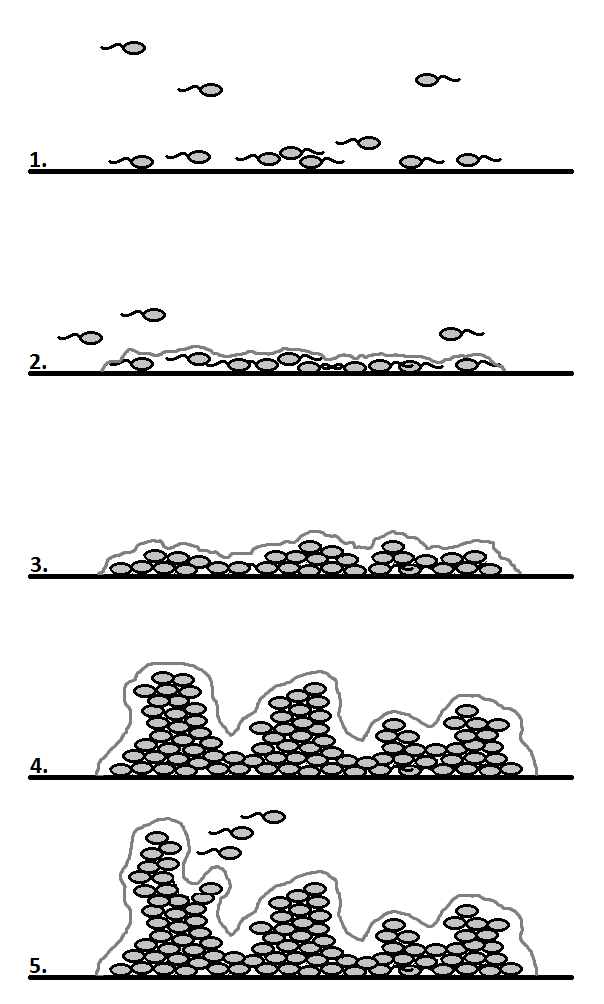
\includegraphics[scale=0.68]{img/biofilm.png}
\caption{Etapy tworzenia się biofilmu;
1. początkowe, odwracalne przyleganie komórek planktonowych do powierzchni,
2. produkcja polimerów zewnątrzkomórkowych (EPS) przez bakterie, w wyniku czego adhezja komórek biofilmu do podłoża staje się nieodwracalna,
3. wczesny rozwój architektury biofilmu,
4. rozwój mikrokolonii w dojrzałym biofilmie, 
5. migracja komórek do otaczającego środowiska;
źródło: opracowanie własne na podstawie B.Kołwzan 2011\cite{kolwzan}}\label{biofilm}
\end{center} 
\end{figure}
\clearpage

Adhezja to istotna cecha bakterii w początkowym etapie zasiedlania, ponieważ rzęski umożliwiają im łatwiejsze odszukanie powierzchni oraz innych komórek, w wyniku czego możliwe jest szybsze tworzenie mikrokolonii. Fimbrie zaś, dzięki obecności grup hydrofobowych, ułatwiają bakterii pokonanie sił odpychania występujących między ujemnie naładowaną ścianą komórkową, a zasiedlaną powierzchnią.
%http://www.pzits.not.pl/docs/Kolwzan.pdf (ostatnie zdanie - przepisane trochę!!!!)
Na etapie adhezji odwracalnej komórki są słabo związane z podłożem (odległości 2-50nm), wykorzystując wiązania hydrofobowe, siły van der Waalsa oraz ruchy Browna\cite{czaczyk, kolwzan}.\

Jeżeli komórki bakterii nie zostaną usunięte odległość między nimi a powierzchnią będzie się zmniejszać, aż przekroczy 1,5nm, a adhezja stanie się nieodwracalna\cite{czaczyk, kolwzan}.
%http://www.pzits.not.pl/docs/Kolwzan.pdf
Dzieje się tak w wyniku oddziaływań pomiędzy znajdującymi się na powierzchni komórki adhezynami a zasiedlaną powierzchnią - powstają wiązania wodorowe oraz kowalencyjne\cite{myszka}.
Kluczową rolę na tym etapie powstawania biofilmu odgrywają wydzielane zewnątrzkomórkowo polimery - EPS(Extracellular Polymeric Substances).\ 
Tworzą one wokół komórek tzw. glikokaliks ułatwiający przyczepianie się komórek do zasiedlanej powierzchni\cite{shi}.\

%SPRAWDZIĆ! Shi X., Zhu X., Biofilm formation and food safetly in food industries, Trends in Food Science and Technology, 20, 407-413, 2009

Następny etap tworzenia się biofilmu stanowi kondycjonowanie powierzchniowe, czyli formowanie się dojrzałego biofilmu poprzez przyłączanie się kolejnych komórek tych samych lub innych mikroorganizmów. Komórki biofilmu regulują ekspresję genów odpowiedzialnych za produkcję polimerów, co przyspiesza rozwój powstałych już mikrokolonii. Wtedy również wewnątrz powstającej struktury kształtują się kanaliki odprowadzające niepotrzebnych metabolitów, a także umożliwiające przesyłanie składników pokarmowych oraz wytwarzanych cząsteczek sygnałowych do mikrokolonii\cite{Lawless, Stankowska, czaczyk-myszka}.\

%czaczyk-myszka: http://m.pfb.info.pl/files/kwartalnik/1_2007/czaczyk-myszka.pdf

%SPRAWDZIĆ!!!!!
%Lawless L., The encyclopedia of essential oils: the complite guideto the use of aromatic oils in aromatheraphy, hebalism, health and well-being, Thorsons, London, 2002
%Stańkowska D., Kaca W., Systemy komunikacji międzykomórkowej bakterii Gram-ujemnych i ich znaczenie w ekspresji cech fenotypowych, Postępy mikrobiologii, 44, 99-111, 2005

Ostatni etap wzrostu biofilmu stanowi rozproszenie się komórek z wierzchniej warstwy biofilmu, w celu zasiedlania nowych powierzchni\cite{czaczyk}.
%\clearpage
\subsection{Czynniki warunkujące oporność biofilmów}

Oporność biofilmów na działanie powszechnie stosowanych dezynfektantów i środków antyseptycznych wynika z szeregu mechanizmów obronnych wykształconych przez komórki tworzące te struktury.\
Poniżej przedstawiono kilka najważniejszych czynników warunkujących oporność biofilmów:

\subsection*{EPS - zewnątrzkomórkowe polimery}

Otoczka bakterii biofilmu, głównie wytwarzane zewnątrzkomórkowo polimery, takie jak białka, fosfolipidy, kwasy nukleinowe czy sacharydy, stanowi swoistą barierę fizyczną przed środkami bakteriobójczymi. Zapewnia również odpowiednie pH i ciśnienie osmotyczne, chroni przed wysuszeniem i uniemożliwia fagocytozę.
Biofilm, dzięki otaczającej go matrycy EPS charakteryzuje się również większą opornością na promienie UV niż takie same komórki w formie planktonu\cite{leginowicz, salek}. 
W zależności od rodzaju ściany komórkowej, EPS mogą być odmiennie naładowane - u bakterii gam-dodatnich polimery mają ładunek dodatni, zaś u bakterii gram-ujemnych mają one charakter anionowy. Ilość i jakość produkowanych zewnątrzkomórkowo polimerów zależna jest od gatunku, bądź gatunków mikroorganizmów tworzących biofilm, jak również od wieku biofilmu, obecności tlenu oraz ilości i rodzaju składników odżywczych\cite{czaczyk-myszka, salek}.


%leginowicz: http://www.eko-dok.pl/2012/39.pdf lub http://www.eko-dok.pl/2012/39.pdf to pochodzi z: Interdyscyplinarne zagadnienia w inżynierii i ochronie środowiska. Tom 2.; Praca zbiorowa pod red. Teodory M. Traczewskiej. Oficyna Wydawnicza Politechniki Wrocławskiej, Wrocław 2012.

%salek: http://www.international-bio-consulting.com/pdf/BIOFILM%20-%20Part%201.pdf -->SAŁEK A., Powstawanie biofilmu w warunkach przemysłowych. CZ. 1. Mechanizm formowania biofilmu i jego struktura, http://www.international-bio-consulting.com/pdf/BIOFILM%20-
%20Part%201.pdf.

\subsection*{Pompy błonowe}
Działanie systemu pomp błonowych polega na rozpoznaniu i usunięciu z matrix komórkowego różnorodnych substancji przeciwdrobnoustrojowych.
Białka tworzące pompy typu efflux w komórce występują pojedynczo lub w grupach i są kodowane w genach zlokalizowanych na chromosomie bakteryjnym, a także na plazmidach.
Bakterie gram-ujemne posiadają pompy  typu RND (Resistance Nodulation cell Division) - białka je kodujące występują tu w potrójnych systemach. Skutecznie usuwają one z komórki wiele różnych związków niepowiązanych chemicznie - antybiotyków, detergentów, barwników czy rozpuszczalników organicznych. Produkcja białek pomp efflux w komórce może być stymulowana obecnością w środowisku subletalnej dawki środka przeciwmikrobiologicznego. Jest ona zależna również od stadium rozwoju danego biofilmu oraz gatunku mikroorganizmów go tworzących\cite{czaczyk-myszka, wasaznik, wiercinska}.

%wiercinska: file:///C:/Users/Asia/Downloads/08-med_dosw_1-2015.pdf
%wasaznik: file:///C:/Users/Asia/Downloads/fulltext661.pdf
%czaczyk-myszka: http://m.pfb.info.pl/files/kwartalnik/1_2007/czaczyk-myszka.pdf

\subsection*{\textit{Quorum sensing}}
\textit{Quorum sensing}, czyli system komunikowania się komórek bakterii w strukturze biofilmu, jest bardzo istotnym zjawiskiem wzmagającym oporność tej struktury.
Komunikacja ta opiera się na wytwarzaniu przez komórki biofilmu określonych związków chemicznych - autoinduktorów, oraz ich wydzielaniu do środowiska. Komórki wytwarzają białka konieczne do odbioru tych sygnałów, dzięki czemu możliwa jest odpowiednia, symultaniczna reakcja zarówno w obrębie jednego gatunku jak i pomiędzy różnymi gatunkami mikroorganizmów\cite{leginowicz}. 
Skutkiem tego systemu komunikacji jest skoordynowana w całej strukturze regulacja ekspresji określonych genów\cite{kolodynski}.
W wyniku różnic w budowie ściany komórkowej bakterii, system \textit{quorum sensing} różni się między bakteriami gram-dodatnimi i gram-ujemnymi.\\
Autoinduktorami u bakterii gram-dodatnich są cząsteczki białkowe, zaś odbieranie sygnału przez komórkę polega na kaskadzie reakcji zapoczątkowanej przez fosforylację kinazy białkowej na skutek kontaktu z cząsteczką sygnałową. Białko regulatorowe, w wyniku szeregu reakcji zostaje ufosforylowane, po czym przyłączając się do danego fragmentu DNA inicjuje transkrypcję określonych genów.\\
W systemie komunikacji bakterii gram-ujemnych autoindukatory stanowią związki niskocząsteczkowe - acetylowane laktony homoseryny (acyl-HSL), które są rozpoznawane i wiązane specyficznie przez białko LuxR. Umożliwia to jego oddziaływanie na sekwencję starterową operonu, w wyniku czego możliwa jest transkrypcja danych genów\cite{czaczyk-myszka, zajac}.
Dodatkowo, cząstki sygnałowe w biofilnie bakterii \textit{Pseudomonas aeruginosa} przemieszczają się w pęcherzykach otoczonych dwuwarstwą lipidową\cite{membrane, smith}\\
Dzięki zjawisku \textit{quorum sensing} możliwa jest regulacja szeregu procesów fizjologicznych biofilmu, co umożliwia korzystniejsze dostosowanie się do zmieniających się warunków środowiska\cite{czaczyk-myszka, leginowicz}.

%membrane: https://www.ncbi.nlm.nih.gov/pubmed/16163359

%smith: https://www.ncbi.nlm.nih.gov/pmc/articles/PMC259138/

%kolodynski: http://direct.dbc.wroc.pl/Content/2109/z18_Kolo.pdf


\subsection{Biofilmy na powierzchniach abiotycznych}
Drobnoustoje tworzące biofilm wykazują zdolność do adhezji zarówno na powierzchniach biotycznych jak i abiotycznych\cite{czaczyk-myszka}.

% !!!!!!!!!!!!!!!!!!! WSTAWIONE !!!!!!!!!!!!!!!!!!!!!!!!!!!!!!!!!!!!!!
Na krzywiznach i w zagłębieniach powierzchni abiotycznych (powstałych w wyniku zarysowań czy pęknięć) kumulują się różnego rodzaju zanieczyszczenia, co ułatwia przyłączanie się komórkom tworzącym biofilm.W przemyśle spożywczym może skutkować to zmianami organoleptycznymi produktu oraz obecnością w nim niepożądanych związków pochodzenia mikrobiologicznego\cite{usuwanie}

%usuwanie: Myszka, K. and Czaczyk, K.  Metody usuwania biofilm(\’o)w bakteryjnych z powierzchni sta(\l)ych  Przemys(\l) Spozywczy  2007  2, s.18-21
 
Podobnie jest w medycynie. Biofilmy tworzą się na różnych szpitalnych przedmiotach i urządzeniach jedno- i wielorazowego użytku. Stwarza to zagrożenie zdrowia pacjentów, często o obniżonej odporności.
Aż 65\% zakażeń występujących u pacjentów szpitali jest skutkiem zdolności mikroorganizmów do wzrastania na powierzchniach abiotycznych\cite{czaczyk-myszka}.\\
Obecność bakterii \textit{Pseudomonas aeruginosa} obserwuje się na cewnikach oddechowych i rurach intubacyjnych, co powoduje choroby płuc, szczególnie u osób chorych na mukowiscydozę.
\cite{mukowiscydoza}
%mukowiscydoza: artykuł:  Sadowska, B. i inni  Cystic fibrosis. Biofilms involved in pulmonary infections  Forum Zakażeń  2013  4(2)
Bakterie te obecne są również na powierzchni cewników moczowych czy kaczek, i mogą wywoływać zapalenia układu moczowo-płciowego\cite{moczowy}.
%moczowy:  Ostrowska, K. i inni  Biofilm bakteryjny jako przyczyna zakaze(‘n) uk(\l)adu moczowego – mikroorganizmy patogenne, metody prewencji i eradykacji  Postepy Hig Med Dosw (online), 2013; 67, s.1027-1033
Biofilm stanowi również poważne zagrożenie w stomatologii. Bakterie \textit{Pseudomonas aeruginosa} były izolowane z wody pochodzącej z układów wodnych unitu stomatologicznego\cite{bzdega}.
%bzdega:  Bzdęga, W. and i inni  The disinfection of water and compressed air systems of a dental unit  Nowiny Lekarskie  2007  76(5)

\section{Olejki eteryczne}

\subsection{Charakterystyka wybranych olejków eterycznych}
Olejki eteryczne dzięki szerokiej gamie właściwości terapeutycznych są coraz chętniej i częściej wykorzystywane w przemyśle kosmetycznym i medycynie. Poniżej przedstawiono charakterystykę 10 wybranych olejków.

%Olejki eteryczne wykorzystane w badaniach wyprodukowane zostały przez firmę Pollena Aroma S.A. z siedzibą w Nowym Dworze Mazowieckim.
Zaliczają się do nich:
\begin{itemize}
\item \textbf{olejek anyżu gwiazdkowego (badianowy)}\\
Olejek ten pochodzi z tropikalnych rejonów Azji, produkowany jest z owoców odmiany wiecznie zielonego anyżku gwiaździstego, \textit{Illicium verum}, naturalnie występującego w północnym Wietnamie oraz w Chinach. Olejek ten pozyskiwany jest w wyniku destylacji owoców z parą wodną\cite{pollena_a, lis}.\\
Głównym składnikiem olejku badianowego jest (E)-anetol, którego zawartość, w zależności od kraju pochodzenia wynosi od 75 do 90$\%$. 
Ponadto, olejek ten zawiera w niewielkich ilościach limonen, linanol, aldehyd anyżowy oraz fenikulinę\cite{lis, Lawrence}. Olejek anyżowy, ze względu na swoje działanie terapeutyczne, wykorzystywany jest w leczeniu stanów zapalnych i nieżycie oskrzeli, czy w jest składnikiem środków rozkurczowych. Olejek stanowi również składnik wielu pastylekpodawanych przy bólu gardła czy syropów wykrztuśnych\cite{lis, deido}.
%"najcenniejsze olejki eteryczne" józef góra anna lis.
% Lawrence: Lawrence B.M. Perf. Flav., 17(2), 49-50, 1992
%deido: Deido I.: Wiad. Ziel. 4, 14-15, 1999

\item \textbf{olejek cynamonowy}\\
Cynamonowce to tropikalne, wiecznie zielone drzewa, których szerokie właściwości cenili sobie już starożytni Egipcjanie, Izraelici, Fenicjanie czy Chińczycy. Olejek cynamonowy może być otrzymywany z kilku odmian tego drzewa, jednak najbardziej rozpowszechnionymi z nich są olejek cynamonowy z kory oraz cynamonowy z liści, produkowane z cynamonowca cejlońskiego (\textit{Cinnamomum zeylanicum}), który uprawiany jest w wielu regionach świata o klimacie tropikalnym lub subtropikalnym takich jak: Brazylia, Antyle, Jamajka, Cejlon, Madagaskar czy Sri Lanka\cite{pollena_c, gorailis}.\\
W zależności od kraju pochodzenia rośliny oraz jej części, jaka wykorzystywana jest do wytworzenia olejku, różni się on składem chemicznym. Głównymi składnikami olejku cynamonowego z kory są aldehyd cynamonowy (31,2-82,1$\%$), eugenol (0,8-13,3$\%$), octan cynamylu (0,3-10,6$\%$) oraz  $\beta$-kariofilen (0,9-4,1$\%$)\cite{gorailis, kedzia2012}.
%kedzia2012: Kędzia A. Aktywność olejku cynamonowego (\textit{Oleum Cinnamoni}) wobec bakterii beztlenowych. Postępy Filoterapii 2012, 2, 67-1

\item \textbf{olejek drzewa herbacianego}\\
Olejek drzewa herbacianego pochodzi z Australii i pozyskiwany jest z rozdrobnionych kłączy kilku gatunków roślin z rodzaju \textit{Melaleuca} na drodze ich destylacji z parą wodną\cite{pollena_d}.
Olejek ten, dzięki swoim właściwościom  przeciwbakteryjnym, przeciwgrzybiczym i oczyszczającym, wykorzystywany jest w kosmetologii oraz w medycynie przy zakażeniach jamy ustnej, infekcjach skórnych i narządów płciowych. Jego działanie sprawia również, iż jest on wykorzystywany w leczeniu infekcji wirusowych\cite{pollena, pollena_d, lis}.\\
Skład jakościowy i ilościowy tego olejku w dużej mierze zależy nie tylko od regionu Australii, ale także od gatunku drzewa herbacianego. Jego skład zmienia się również wraz z czasem jego przechowywania. Związkami charakterystycznymi dla tej grupy olejków są monoterpeny takie jak: terpinen-4-ol, $\gamma$-terpinen, $\alpha$-terpineol, $\alpha$-pinen oraz limomen\cite{Kreck, lis}.

%pollena_d: http://www.drbeta.pl/olejek-drzewa-herbacianego.html
% pollena: http://pollenaaroma.com.pl/wp-content/uploads/2015/04/Beauty-Forum-12-2013-Najcenniejsze-olejki-eteryczne.pdf
% Kreck M. i wsp.: Flavour Fragr. J., 17(1), 32-40, 2002

\item \textbf{olejek goździkowy}\\
Goździkowiec korzenny (\textit{Eugenia caryophyllata}), z którego pąków kwiatowych produkowany jest olejek goździkowy, to pochodzące z Indonezji wiecznie zielone drzewo. Goździki o intensywnym smaku i korzennym zapachu wykorzystywane są w kuchni jako przyprawa, jak również stanowią surowiec leczniczy, np. jako środek zwiększający apetyt i poprawiający trawienie. Olejek goździkowy dzięki swoim właściwościom przeciwbólowym i antyseptycznym wchodzi w skład produktów stomatologicznych oraz maści przeciwbólowych wykorzystywanych w leczeniu stawów\cite{brud1992, gorailis}.\\
Głównym składnikiem olejku goździkowego jest eugenol, jednak jego zawartość znacznie różni się w zależności od kraju pochodzenia rośliny i waha się od 35 do 90$\%$. Pozostałe istotne związki to octan eugenylu, $\beta$-kariofilen czy $\alpha$-humulen\cite{gorailis}.

%brud1992: Brud W.S., Konopacka I.: Pachnąca apteka, Comes, Warszawa, 47-48, 1992

\item \textbf{olejek hyzopowy}\\
Olejek hyzopowy pozyskuje się z popularnego w Azji Środkowej i Europie Południowej ziela hyzopu lekarskiego, w wyniku jego destylacji z parą wodną. Olejek ten ma korzystny wpływ na układ pokarmowy człowieka poprzez pobudzanie wydzielania kwasów żołądkowych oraz poprawę perystaltyki jelit. Odznacza się również  właściwościami dezynfekującymi oraz uśmieża ból, dzięki czemu wykorzystywany jest w płukankach stosowanych podczas stanów zapalnych jamy ustnej czy w okładach na rany. Dzięki słodkiemu, kwiecistemu  zapachowi wykorzystywany jest równieżw przemyśle kosmetycznym\cite{gorailis, ruminska}.\\
Skład chemiczny olejku w dużej mierze zależy od pochodzenia wykorzystywanej do jego wytworzenia rośliny. Wspólną dla olejków z różnych krajów grupą związków są dicykliczne ketony: pinokamfon(do 12,6$\%$), izopinokamfon(do 54,3$\%$) oraz pinokarwon(do 20,3$\%$). W olejku pochodzenia francuskiego dominuje linanol, w olejku hiszpańskim 1,8-cyneol, zaś w czarnogórskim - limonen\cite{gorailis}.

%ruminska: Rumińska A., Ożarowski A.: Leksykon roślin leczniczych, PWRiL, Warszawa, 175, 1980

\item \textbf{olejek kanuka}\\
Olejek kanuka wytwarza się z liści i gałązek wiecznie zielonego białego drzewa herbacianego - \textit{Kunzea ericoides}, występującego naturalnie w Nowej Zelandii i Australii\cite{lis}. Olejek ten ma właściwości bójcze w stosunku do bakterii gram-dodatnich, a także działa przeciwbólowo, przez co wykorzystywany jest w kompresach w leczeniu reumatyzmu czy żylaków\cite{pollena_k, brud2001}.\\
Głównym składnikiem olejku kanuka jest $\alpha$-pinen, którego ilość wynosi od 55,5 do 74,8$\%$. Wśród pozostałych składników wyróżnia się również p-cymen(3,4-12,6$\%$) oraz 1,8-cyneol(3,2-6,2$\%$)\cite{manukaikanuka, lis}.

%pollena_d: http://www.drbeta.pl/olejek-kanuka.html
%brud2001: Brud W.S., Konopacka I.: Pachnąca apteka, Pagina, Warszawa, 80, 2001
%gniewosz: Gniewosz M. i wsp.: Porównanie działania przeciwdrobnoustrojowego olejków eterycznych manuka(\textit{Leptospermum scoparium}) i kanuka(\textit{Kunzea ericoides}), Bromatologia i Chemia Toksykologiczna, 3, 639-644, 2012
\clearpage
\item \textbf{olejek manuka}\\
Olejek manuka pozyskiwany jest w wyniku destylacji z parą wodną świeżych lub podsuszonych liści czerwonego drzewa herbacianego - Manuka (\textit{Leptospermum scoparium}). Krzew ten występuje naturalnie w Nowej Zelandii, Australii, Tasmanii oraz południowej części Azji. Olejek wykazuje działanie przeciwdrobnoustrojowe oraz przeciwbólowe, dlatego też wykorzystywany jest w leczeniu chorób skóry w formie okładów, czy w leczeniu podrażnienia górnych dróg oddechowych poprzez inhalacje\cite{lis, pollena_ma}.\\
Odmiany manuki, z których produkowany jest olejek, są, obok regionu uprawy,  ważnym czynnikiem, znacząco różnicującym olejki pod kątem składu chemicznego. 
Każda odmiana olejku manuka zawiera $\alpha$-pinen (0,5-63$\%$), 1,8-cyneol, endusmol oraz leptospermon - związek charakterystyczny dla tego surowca\cite{manukaikanuka, lis}.


\item \textbf{olejek mięty pieprzowej}\\
Olejek mięty pieprzowej produkowany jest z części nadziemnej pospolitej w Europie byliny - \textit{Mentha Piperita}\cite{pollena_mi}. Wykazuje właściwości chłodzące, znieczulające, łagodzi podrażnienia, działa rozkurczowo i uspokajająco. To oraz ożeźwiający aromat sprawiają, iż jest on jednym z najbardziej rozpowszechnionych i najczęściej stosowanych w medycynie i aromaterapii olejków eterycznych\cite{pollena, gorailis}.\\
Dominującym składnikiem olejku miętowego jest mentol, którego zawartość, w zależności od regionu i warunków uprawy, waha się między 24,1 do 59,4$\%$. Ważnym składnikiem olejku jest menton, występujący w ilościach od 4,6 do 32,1$\%$\cite{Law}.

%Law: Lawrence B.M.: Perf. Flav., 18(4), 59-71, 1993
%Chłodzące, antybakteryjne, łagodzące podrażnienia,
%pollena_mi: http://www.drbeta.pl/olejek-miety-pieprzowej.html

\item \textbf{olejek tymiankowy}\\
Olejek tymiankowy może być wytwarzany z jednej z dwóch roślin pochodzących z rejonu Morza Śródziemnego: z formy francuskiej lub niemieckiej tymianku pospolitego - \textit{Thymus vulgaris} lub z tymianku hiszpańskiego - \textit{Thymus zygis}. Ziele tymianku zebrane w fazie kwitnienia wykorzystywane jest w przemyśle spożywczym jako przyprawa, oraz w przemyśle farmaceutycznym i w aromaterapii do produkcji olejku eterycznego. Najważniejszymi właściwościami olejku tymiankowego są działanie bakteriobójcze, a także działanie wykrztuśne i pozytywny wpływ na układ trawienny, poprzez pobudzanie wytwarzania kwasów żółciowych\cite{lis}.\\
Skład olejku tymiankowego różni się między poszczególnymi chemotypami tej rośliny. W każdym rodzaju obecny jest tymol (od 0,5 do 83,2$\%$), a także karwakrol, p-cymen i linanol\cite{Lawr, lis}.

%Lawr: Lawrence B.M.,Perf. Flav., 17(5), 140-143, 1992

\item \textbf{olejek ylangowy (ylang-ylang})\\
Nazwa tego olejku wywodzi się z potocznej nazwy jagodinu wonnego (\textit{Cananga odorata}) - tropikalnego drzewa pochodzącego z Filipin. Jego pachnące, żółte kwiaty stanowią surowiec do produkcji olejku, po porannych zbiorach niezwłocznie poddawane są destylacji z parą wodną. 
Dzięki swojemu tropikalnemu, kwiatowemu, słodkiemu zapachowi olejek ylang-ylang stosowany jest na szeroką skalę w przemyśle perfumeryjnym\cite{gorailis}. 
Ponadto, uważany jest za afrodyzjak, a w aromaterapii wykorzystywany jest w leczeniu depresji i nerwic\cite{pollena_y}. 
Olejek ten wykazuje aktywność przeciwgrzybiczą\cite{hammer}. Ma również właściwości przeciwdrobnoustrojowe, ze względu na obecność takich związków jak kwas benzoesowy, alkohole terpenowe - linalol i geraniol, czy monoterpen - $\alpha$-pinen\cite{kedzia_ylang}. 

%kedzia_ylang: Kędzia A. Działanie olejku ylangowego na bakterie beztlenowe w obrębie zakażeń jamy ustnej. Postępy Filoterapii 2008, 1, 15-19 http://www.czytelniamedyczna.pl/2596,dzialanie-olejku-ylangowego-na-bakterie-beztlenowe-wyodrebnione-z-zakazen-jamy-u.html


%hammer: Hammer KA, Carson CF, Riley TV. Antimicrobial activity of essential oils and other plant extracts. J Appl Microbiol 1999; 86:985-90. - http://onlinelibrary.wiley.com/doi/10.1046/j.1365-2672.1999.00780.x/full

%thompson: https://www.ncbi.nlm.nih.gov/pmc/articles/PMC4220539/
%Aseptyczne, przeciwzapalne, zapobiega wypadaniu włosów i przetłuszczaniu skóry, przeciwstresowe \cite{pollena}
%pollena_y: duże zróżnicowanie ---- http://pollenaaroma.com.pl/pl/kosmetyka-i-aromaterapia/oferta/ 

\end{itemize}

\clearpage

\subsection{Działanie olejków eterycznych na biofilm bakteryjny}
Przeciwdrobnoustrojowe właściwości olejków eterycznych oraz ekstraktów roślinnych znane są ludzkości od stuleci. Współcześnie, z uwagi na zwiększającą się lekooporność szczepów tworzących biofilm, poszukuje się alternatywnych, skutecznych środków o aktywności biobójczej, również wśród tych, pochodzenia naturalnego\cite{budzynska, hammer, budzynska3}. Wzrasta także zainteresowanie terapią łączącą antybiotyki z substancjami naturalnymi - olejkami eterycznymi lub pochodzącymi z nich związkami\cite{budzynska3, budzynska2}.\\
%\clearpage
Olejki eteryczne wykazują działanie hamujące rozwój biofilmów bakterii gram-dodatnich, gram-ujemnych czy grzybów. Wykazano znaczące działanie bakteriobójcze olejku goździkowego wobec bakterii \textit{Staphylococcus aureus} oraz \textit{Candida albicans}\cite{budzynska3}. Wobec bakterii \textit{Pseudomonas aeruginosa} działanie hamujące wykazał dodatek olejku lawendowego do badanej emulsji, zaś olejek cedrowy wykazuje silne działanie przeciwgrzybicze wobec biofilmów gatunku \textit{Candida parapsilosis} i \textit{C. utilis}\cite{kom_adaszynska}.

Związki roślinne posiadają zdolność do oddziaływania na strukturę biofilmu i niektóre mechanizmy stanowiące o jego oporności, czego przykładem może być olejek drzewa herbacianego. 
Jego działanie polega na dziurawieniu błon biologicznych komórek bakterii powodując jej przepuszczalność, w wyniku czego zaburzona jest homeostaza komórek, a w konsekwencji następuje ich śmierć\cite{drzewo1}. Podobny mechanizm działania wykazuje mentol - składnik olejku miętowego, a także olejek tymiankowy i lawendowy\cite{kom_trytek}.\\



%Wyciągi roślinne oraz olejki eteryczne mogą znaleźć zastosowanie również w leczeniu wirusa HSV-1 i HSV-2 - wirusa opryszczki pospolitej (\textit{herpes simplex virus}). Olejki niszczą powłokę wirusa, uniemożliwiając...

%kom_adaszynska: komórka plik Adaszynska.p...

%manuka i kanuka: file:///C:/Users/Asia/Desktop/manuka%20i%20kanuka.pdf

%budzynska3: file:///C:/Users/Asia/Downloads/06-med_dosw_4-2011%20(3).pdf

%budzynska2: http://www.vetpol.org.pl/dmdocuments/06_Potencjalne%20wykorzystanie.pdf

%budzynska: http://dspace.uni.lodz.pl:8080/xmlui/handle/11089/9046

%Hammer KA, Carson CF, Riley TV. Antimicrobial activity of essential oils and other plant extracts. J Appl Microbiol 1999; 86:985-90. - 

%hammer: Hammer KA, Carson CF, Riley TV. Antimicrobial activity of essential oils and other plant extracts. J Appl Microbiol 1999; 86:985-90. - http://onlinelibrary.wiley.com/doi/10.1046/j.1365-2672.1999.00780.x/full

%thompson: https://www.ncbi.nlm.nih.gov/pmc/articles/PMC4220539/






\chapter{Cel i zakres pracy}

%Celem pracy była ocena autentyczności badanych miodów pszczelich pod kątem ich profilu zapachowego oraz wybranych właściwości fizykochemicznych.

Celem pracy była ocena zdolności wybranych bakterii z rodzaju \textit{Pseudomonas} do tworzenia biofilmów na powierzchni cewników medycznych w obecności olejków eterycznych.

%Zakres pracy obejmował analizę fizykochemiczną miodów pszczelich (zawartość wody, stężenie substancji nierozpuszczalnych w wodzie oraz kwasowość), a także oznaczenie profilu związków lotnych przy użyciu metody HS-SPME-GC/MS.

W badaniach została określona ilość tworzącego się biofilmu oraz dynamika jego wzrostu, w obecności wybranych olejków eterycznych w stężeniu 1/2 oraz 1/4 wartości najmniejszego stężenia hamującego.

%[...DOK!!!!!...]

\chapter{Materiały}

\section{Materiał biologiczny i techniczny}

W przeprowadzonych badaniach materiał badawczy stanowiło sześć szczepów bakterii należących do rodzaju \textit{Pseudomonas}, przedstawionych w tabeli poniżej.
Bakterie \textit{Pseudomonas aeruginosa} ATTC 15442 pochodziły z American Type Culture Collection, zaś pozostałe 5 szczepów zostały wcześniej wyizolowane ze środków kosmetycznych.\\


\begin{table}[h!]
\centering
\caption{Badane mikroorganizmy}
\label{my-label}
\begin{tabular}{|c|c|c|}
\hline
\textbf{Szczep}                                  & \textbf{Oznaczenie} & \textbf{Pochodzenie}                                                               \\ \hline
\multirow{3}{*}{\textit{Pseudomonas aeruginosa}} & ATCC 15442          & American Type Culture Collection                                                   \\ \cline{2-3} 
                                                 & CF II               & \multirow{2}{*}{Środki kosmetyczne}                                                \\ \cline{2-2}
                                                 & CF V                &                                                                                    \\ \hline
\multirow{3}{*}{\textit{Pseudomonas cedrina}}    & PC                  & American Type Culture Collection                                                   \\ \cline{2-3} 
                                                 & DH1                 & \multirow{2}{*}{\begin{tabular}[c]{@{}c@{}}Dehyquart\textsuperscript{\textregistered}\\ (BASF Niemcy)\end{tabular}} \\ \cline{2-2}
                                                 & DH2                 &                                                                                    \\ \hline
\end{tabular}
\end{table}
źródło: opracowanie własne
\clearpage

W badaniach wykorzystano 10 olejków eterycznych  firmy Pollena Aroma S.A. z siedzibą w Warszawie, które zestawiono poniżej:
\begin{itemize}
\item olejek anyżowy (\textit{Illicium verum Oil})
\item olejek cynamonowy (\textit{Cinnamomum Zeylanicum Bark Oil})
\item olejek drzewa herbacianego (\textit{Melaleuca Alternifolia Oil})
\item olejek goździkowy (\textit{Eugenia Caryophyllus Oil})
\item olejek hyzopowy (\textit{Citrus Grandis Oil})
\item olejek kanuka (\textit{Kunzea Ericoides Oil})
\item olejek manuka (\textit{Leptospermum Scoparium Oil})
\item olejek mięty pieprzowej (\textit{Mentha Piperita Oil})
\item olejek tymiankowy (\textit{Thymus Vulgaris Oil})
\item olejek ylang-ylang (\textit{Cananga Odorata Flower Oil})\\
\end{itemize}
Olejki przechowywane były w lodówce, w temperaturze ok. 4\degree C, w ciemnych buteleczkach.
\clearpage

W badaniach wzrost biofilmu prowadzono na 1cm fragmentach cewnika oddechowego firmy Unomedical o długości całkowitej 60cm. Wymiary fragmentów cewnika (katetera) przedstawiono na Rys.\ref{stent}.\
\begin{figure}[!h]
\begin{center}
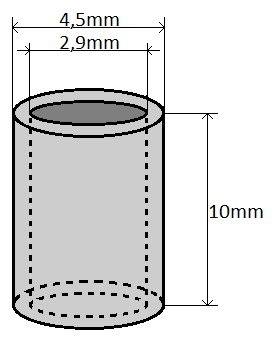
\includegraphics[scale=0.6]{img/stent.png}
\caption{Wymiary wykorzystywanych w badaniach fragmentów cewników oddechowych; źródło: opracowanie własne}\label{stent}
\end{center} 
\end{figure}
\section{Pożywki i odczynniki}
W badaniach stosowano płynną pożywkę TSB (Tryptone Soya Broth). Do obmywania kateterów po inkubacji oraz do ich przechowywania wykorzystywano fizjologiczny roztwór soli.
% tsb:  http://www.merckmillipore.com/INTERSHOP/web/WFS/Merck-DE-Site/de_DE/-/EUR/ShowDocument-File?ProductSKU=MDA_CHEM-146316&DocumentId=146316_SDS_PL_PL.PDF&DocumentType=MSD&Language=PL&Country=PL&Origin=SERP.


\begin{table}[h!]
\centering
\caption{Stosowane pożywki i odczynniki}
\label{my-label}
\begin{tabular}{|c|c|}
\hline
\textbf{Podłoże/Odczynnik}                                                     & \textbf{Składniki}         \\ \hline
\multirow{4}{*}{\begin{tabular}[c]{@{}c@{}}TSB\\ (Merck, Niemcy)\end{tabular}} & Pepton K 15,0g             \\ \cline{2-2} 
                                                                               & Pepton SP 5,0g             \\ \cline{2-2} 
                                                                               & NaCl 5,0g                  \\ \cline{2-2} 
                                                                               & Woda destylowana do 1000ml \\ \hline
\multirow{2}{*}{Fizjologiczny roztwór soli}                                    & NaCl 8,5g                  \\ \cline{2-2} 
                                                                               & Woda destylowana do 1000ml \\ \hline
\end{tabular}
\end{table}
źródło: karta charakterystyki TSB\cite{tsb}, opracowanie własne

\chapter{Metody badań}
\section{Sposób oznaczenia zdolności tworzenia biofilmu na powierzchni cewników oddechowych}\label{pierwotna}

Pierwotnie opracowaną metodykę oznaczenia zdolności tworzenia biofilmu przez bakterie \textit{Pseudomonas} przeprowadzono dla szczepu ATTC 15442 w obecności olejków: cynamonowego, goździkowego, mięty pieprzowej i tymiankowego, w stężeniach odpowiadających 1/2 oraz 1/4 ich minimalnego stężenia hamującego dla tych bakterii (dane niepublikowane, Zabielska, 2017).\

Z prowadzonej w płynnej pożywce TSB 24-godzinnej hodowli badanego szczepu bakterii pobierano 0,5ml i przenoszono do butelek, zawierających 50ml pożywki TSB oraz uprzednio przygotowane, pocięte na równe, 1-centymetrowe odcinki standardowe oraz silikonowe cewniki oddechowe. 
Tak przygotowane hodowle inkubowano w temperaturze 30\degree C przez pół godziny, po czym do wszystkich poza próbką kontrolną dodano olejki eteryczne w odpowiednich stężeniach, zgodnie ze schematem \ref{metoda_pierwotna}.
Tak otrzymane hodowle w butelkach inkubowano w temperaturze 30\degree C.
Próbki pobierano po 0,5; 2; 4; 8 oraz 24 godzinach inkubacji.

\clearpage
\begin{figure}[!h]
\begin{center}
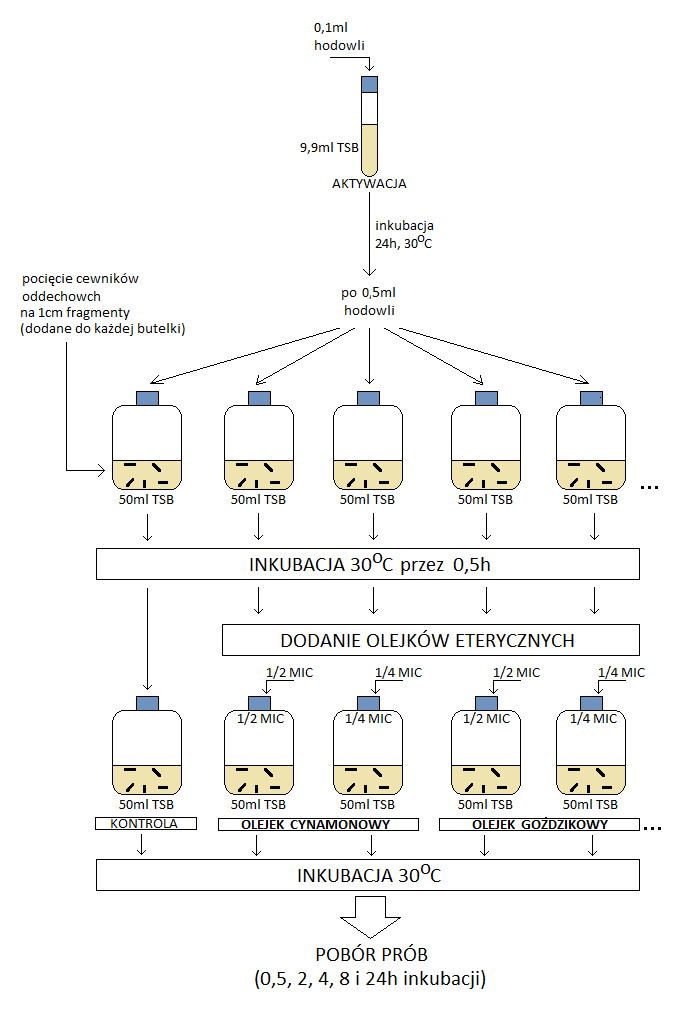
\includegraphics[scale=0.72]{img/mgr_metodyka_stara.png}
\caption{Procedura hodowli biofilmu bakteryjnego\\
źródło: opracowanie własne}\label{metoda_pierwotna}
\end{center} 
\end{figure}
\clearpage

Pobór próbek każdorazowo składał się z trzech części:
\begin{enumerate}
\item z każdej z prowadzonych hodowli pobierano 1ml zawiesiny w 4 powtórzeniach,
\item z każdej hodowli pobierano 4 katetery z cewnika standardowego, 
\item z każdej hodowli pobierano 4 katetery z cewnika silikonowego.
\end{enumerate}
Pobrane fragmenty cewników obmywano 2ml fizjologicznego roztworu soli, w celu pozbycia się luźno zaadherowanych komórek, po czym przenoszono każdy z nich do 1ml roztworu fizjologicznego soli.

W celu oddzielenia komórek biofilmu próbki z fragmentami cewnika poddano sonifikacji za pomocą homogenizatora ultradźwiękowego przy trybie pracy pulsacyjnym (częstotliwość=1, amplituda=1, czas=60s). Podczas sonifikacji, próbki schładzano poprzez umieszczenie ich w pojemniku z lodem.
Dla wszystkich zawiesin zmierzono absorbancję spektrofotometrem przy długości fali $\lambda = 540nm$(Rys.\ref{pomiar_stare}). Dla zawiesiny bakterii pomiar wykonano wobec pożywki TSB, zaś dla próbek zawierających fragmenty cewników wobec wody destylowanej.\
Liczbę komórek odpowiadającą otrzymanym wartościom absorbancji wyliczono z krzywych kalibracyjnych (dane niepublikowane, Zabielska, Kunicka-Styczyńska, 2017), po czym przeliczono na 1cm$^2$ powierzchni cewnika oddechowego.
\begin{figure}[!h]
\begin{center}
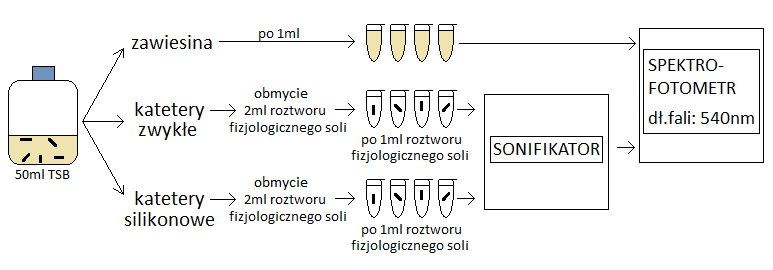
\includegraphics[scale=0.65]{img/pomiar_stare.png}
\caption{Procedura przygotowania próbek do określenia poziomu biofilmu\\
źródło: opracowanie własne}\label{pomiar_stare}
\end{center} 
\end{figure}

\clearpage
\section{Zmodyfikowana metodyka oznaczania zdolności tworzenia biofilmu na powierzchni cewników oddechowych}

Oznaczanie zdolności tworzenia biofilmu przez bakterie \textit{Pseudomonas} prowadzono w obecności olejków eterycznych w stężeniach równych 1/2 oraz 1/4 wartości najmniejszego stężenia hamującego(MIC) obliczonego dla danego szczepu (dane niepublikowane, Zabielska, 2017).
Jeden cykl procesu wykonywano dla jednego szczepu mikroorganizmu oraz 10 olejków eterycznych w dwóch powyższych stężeniach.\

Z prowadzonej w płynnej pożywce TSB 24-godzinnej hodowli badanego szczepu bakterii pobierano 0,8ml i przenoszono do butelki, zawierającej 80ml pożywki TSB oraz uprzednio przygotowane, pocięte na równe, 1-centymetrowe odcinki cewniki oddechowe.
Tak przygotowaną hodowlę inkubowano w temperaturze 30\degree C przez 4 godziny.\
Po upływie tego czasu, każdy fragment kateteru pobierano z hodowli pęsetą, po czym obmywano go 2ml fizjologicznego roztworu soli, w celu usunięcia luźno zaadherowanych komórek, i umieszczano w butelkach zawierających 20ml pożywki TSB oraz dodaną uprzednio odpowiednią ilość olejków eterycznych do końcowego stężenia 1/2 oraz 1/4 MIC.
W każdym cyklu procesu, oprócz butelek zawierających olejki eteryczne, wykonywano również próbkę kontrolną, zawierającą jedynie 20ml płynnej pożywki TSB.
Tak otrzymane 21 hodowli w butelkach inkubowano w temperaturze 30\degree C.
Próbki pobierano po 8, 24, 48 oraz 72 godzinach inkubacji(Rys.\ref{proces_badawczy}).

\clearpage
\begin{figure}[!h]
\begin{center}
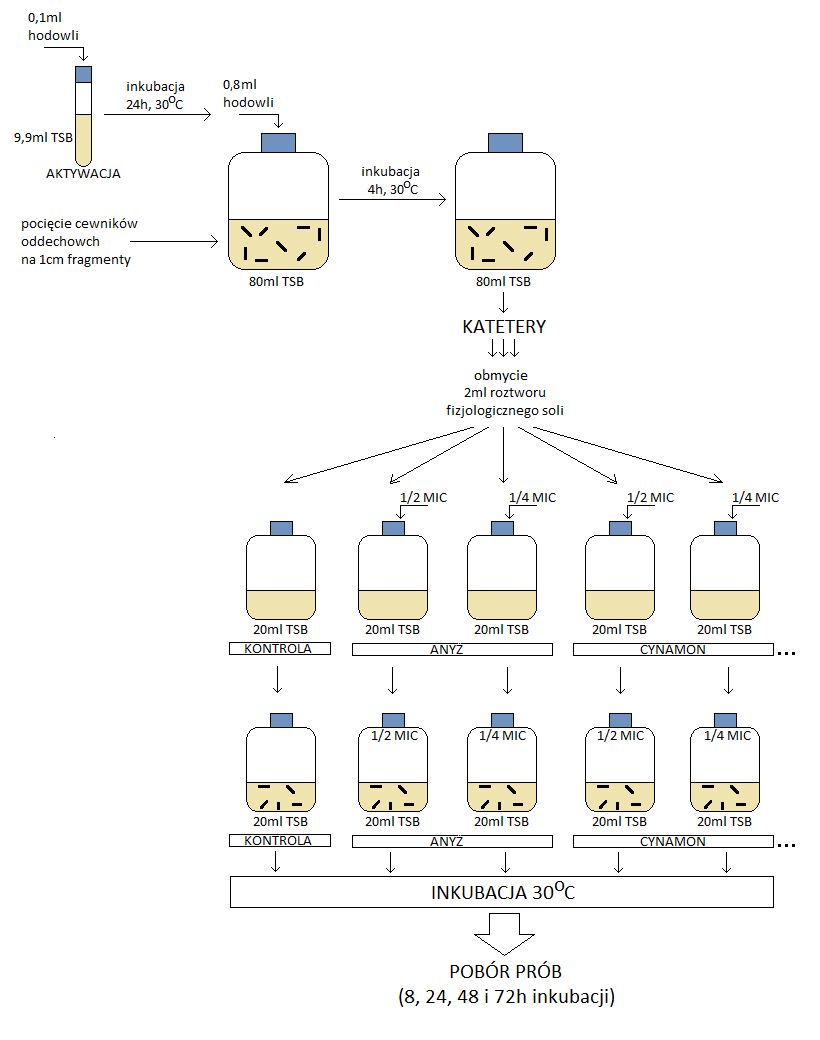
\includegraphics[scale=0.75]{img/mgr_metodyka.png}
\caption{Zmodyfikowana procedura hodowli biofilmu bakteryjnego\\
źródło: opracowanie własne}\label{proces_badawczy}
\end{center} 
\end{figure}
\clearpage

Każdy pobór próbek składał się z dwóch części:
\begin{enumerate}
\item z każdej hodowli pobierano 1ml zawiesiny w czterech powtórzeniach,
\item z każdej hodowli pobierano 4 katetery i po obmyciu zawieszono każdy w 1ml fizjologicznego roztworu soli.
\end{enumerate}

Dalsze postępowanie z próbkami było analogiczne jak przedstawiono w punkcie \ref{pierwotna}.
%\autoref{sec:Pierwotna metodyka}

%\begin{figure}[!h]
%\begin{center}
%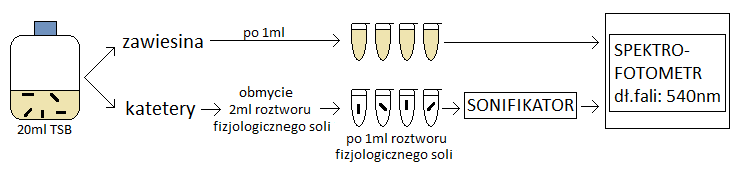
\includegraphics[scale=0.75]{img/pomiar.png}
%\caption{Schemat stosowanego poboru i pomiaru prób\\
%źródło: opracowanie własne}\label{pomiar}
%\end{center} 
%\end{figure}

\section{Obliczenia i analiza statystyczna wyników}
Z uzyskanych wartości absorbancji, dla próbek zawierających fragmenty cewników,  wyliczono odpowiadającą im liczbę komórek (z krzywych kalibracyjnych - dane niepublikowane, Zabielska, Kunicka-Styczyńska). Otrzymane wartości przeliczono na 1 cm$^2$ powierzchni cewnika, po czym wyliczono średnią arytmetyczną, zgodnie ze wzorem:
\begin{equation}
\bar{x}=\frac{1}{N}\sum_{i=1}^N x_i
\end{equation}
gdzie:

N - liczba wykonanych pomiarów,

i - numer kolejnego pomiaru.\\
Odchylenie standardowe stanowiące miarę zmienności mierzonej wartości wokół średniej arytmetycznej wyznaczono według wzoru:

\begin{equation}
s=\sqrt{\frac{1}{N-1}\sum_{i=1}^N(x_i-\bar{x})^2}
\end{equation}
gdzie:

N - liczba wykonanych pomiarów,

i - numer kolejnego pomiaru,

$\bar{x}$ - średnia arytmetyczna.\\

\chapter{Omówienie wyników}

%DYSKUSJA: 
%http://www.cmdr.ubc.ca/trainingprogram/Papers%202006%202007/jp_Feb25b_08.pdf
%
%
%
W niniejszej pracy zbadano zdolność sześciu wybranych szczepów bakterii z rodzaju \textit{Pseudomonas} do tworzenia biofilmu na powierzchni cewników medycznych w obecności dziesięciu olejków eterycznych, dodanych w stężeniach odpowiadających 1/2 oraz 1/4 wartości MIC. Każdorazowo pomiar wykonywano w czterech powtórzeniach.
Określono dynamikę tworzenia biofilmu, a także dynamikę wzrostu wybranych bakterii w formie planktonu w podanych warunkach.
W celu porównania otrzymanych wyników dla każdego szczepu równocześnie wykonywano próbę kontrolną, oznaczaną na poniższych wykresach kolorem granatowym.
%Wykonano także zdjęcia mikroskopowe uzyskanych preparatów.
%(jak to opisać?)

\clearpage

\section{Dynamika tworzenia biofilmu bakteryjnego w obecności olejków eterycznych}

\subsection{Bakterie \textit{Pseudomonas aeruginosa} ATCC 15442} 

Biomasa w próbce kontrolnej w pierwszych dwóch dobach prowadzenia hodowli przyrasta równomiernie i w 48 godzinie osiąga wartość rzędu 10$^8$jtk/cm$^2$, która utrzymuje się w trzeciej dobie hodowli.\\
W większości hodowli szczepu ATCC 15442 prowadzonych w pożywce TSB z dodatkiem olejków eterycznych zaobserwowano spowolniony wzrost biomasy wzrastającej na cewnikach medycznych, w stosunku do próby kontrolnej.
Największe działanie spowalniające przyrost biomasy tych bakterii zaobserwowano w przypadku hodowli z dodatkiem olejku hyzopowego, zarówno w stężeniu 1/2 jak i 1/4 MIC, olejku mięty pieprzowej w stężeniu odpowiadającemu 1/2 MIC jak i z dodatkiem olejku drzewa herbacianego w stężeniu 1/4 MIC.\\
Dynamika wzrostu badanego szczepu w hodowlach z dodatkiem olejku anyżowego z stężeniu 1/4 MIC, olejku goździkowego w 1/4 MIC oraz olejku ylangowego w stężeniu 1/2 MIC była zbliżona do dynamiki zaobserwowanej w próbie kontrolnej, co może świadczyć o znikomym wpływie tych dodatków na rozwój biofilmu bakterii ATCC 15442.\\
W przypadku hodowli z dodatkiem olejku kanuka (1/2 oraz 1/4 MIC), manuka (1/2 i 1/4 MIC) oraz olejku ylangowego w stężeniu 1/2 MIC w ciągu pierwszej doby poziom biomasy był zbliżony do poziomu biomasy w próbie kontrolnej. W drugiej i trzeciej dobie poziom biomasy utrzymuje się na stałym poziomie - rzędu 10$^4$-10$^5$jtk/cm$^2$, co może świadczyć o tym, iż dodatek tych olejków, przy wydłużonym czasie kontaktu ogranicza przyrost biomasy biofilmu. 
\clearpage

\begin{figure}[!h]
\begin{center}
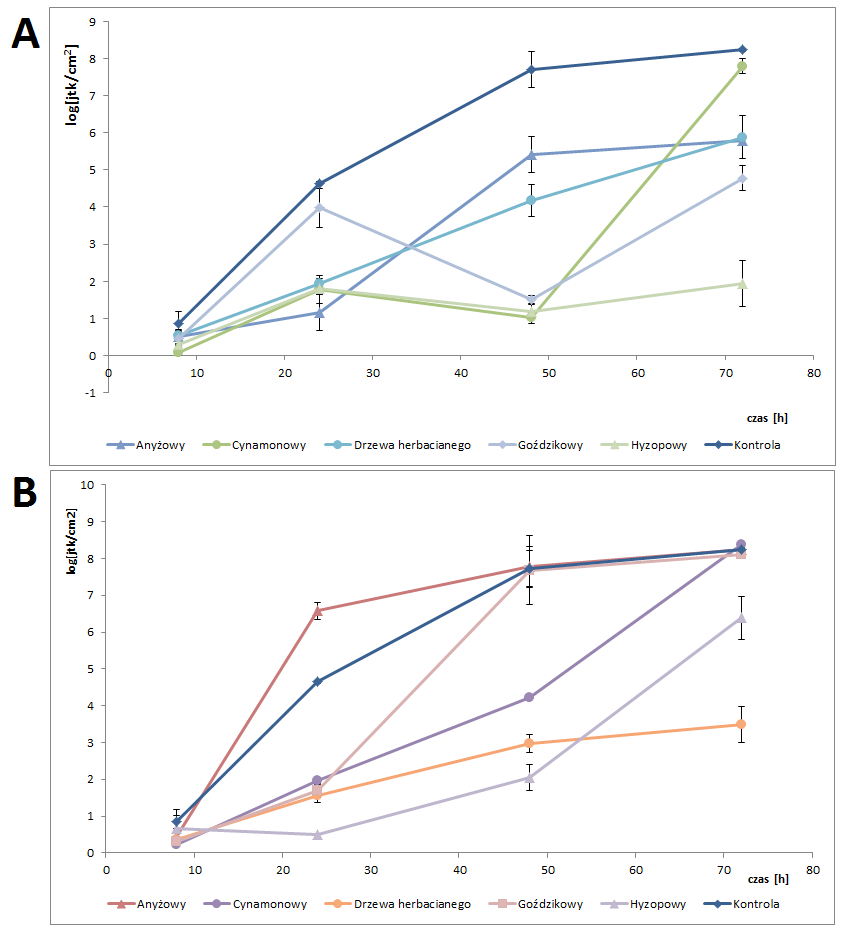
\includegraphics[scale=0.7]{img/ref-a.png}
\caption{Dynamika tworzenia biofilmu bakterii \textit{Pseudomonas aeruginosa} ATCC 15442 w obecności olejku anyżowego, cynamonowego, drzewa herbacianego, goździkowego i hyzopowego w ilości odpowiadającej A - 1/2 MIC; B - 1/4 MIC.}\label{ref-a}
\end{center} 
\end{figure}

\begin{figure}[!h]
\begin{center}
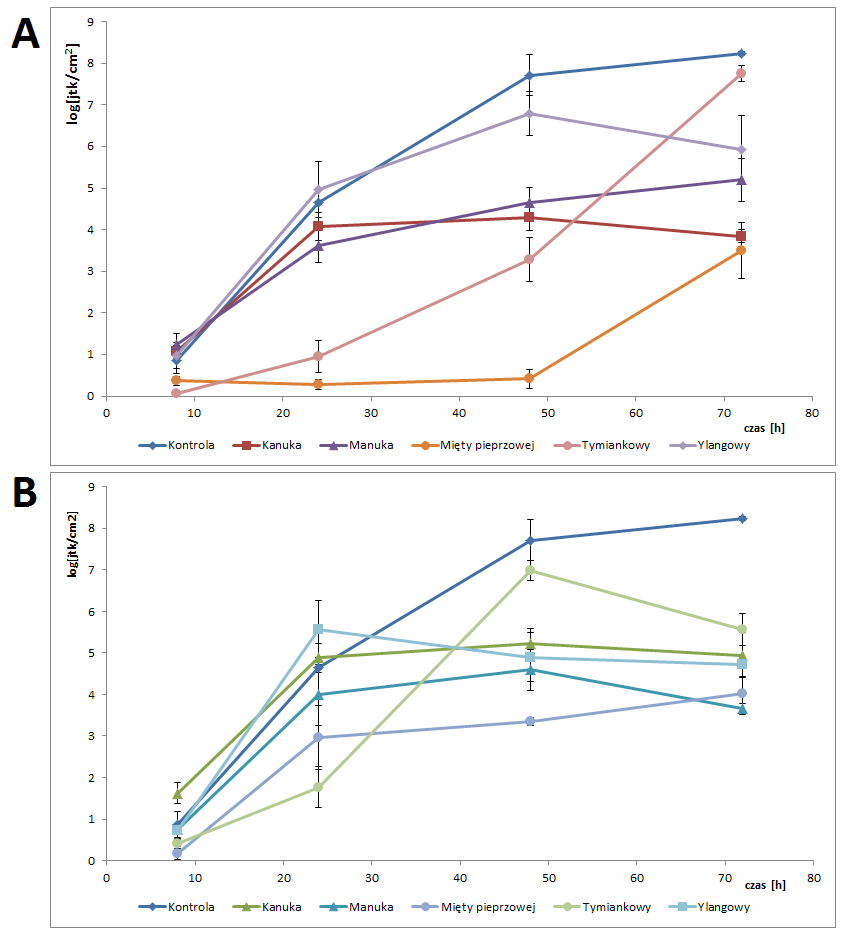
\includegraphics[scale=0.7]{img/ref-b.png}
\caption{Dynamika tworzenia biofilmu bakterii \textit{Pseudomonas aeruginosa} ATCC 15442 w obecności olejku kanuka, manuka, mięty pieprzowej, tymiankowego i ylangowego w ilości odpowiadającej A - 1/2 MIC; B - 1/4 MIC.}\label{ref-b}
\end{center} 
\end{figure}
\clearpage

\subsection{Bakterie \textit{Pseudomonas aeruginosa} CFII}
Biomasa biofilmu w próbce kontrolnej przyrasta niemal liniowo, osiągając w 72. godzinie hodowli wartość rzędu 10$^4$.
Komórki biofilmu szczepu CFII w tych samych warunkach namnażają się zdecydowanie mniejszym tempie niż komórki szczepu referencyjnego ATCC 15442.\\
W hodowlach z dodatkiem olejku anyżowego w stężeniu odpowiadającemu 1/2 wartości MIC, olejku drzewa herbacianego (1/2 MIC), goździkowego (1/4 MIC) oraz tymiankowego w stężeniu 1/2 i 1/4 MIC zaobserwowano podobną dynamikę wzrostu jak w próbie kontrolnej, jednak wartości ilościowe jtk/cm$^2$ w danym punkcie pomiarowym były o rząd wielkości mniejsze, co wskazywać może na umiarkowane działanie hamujące rozwój biofilmu bakterii szczepu CFII.\\
W hodowlach z dodatkiem olejku hyzopowego w stężeniu odpowiadającemu 1/2 MIC, drzewa herbacianego (1/4 MIC) oraz olejku mięty pieprzowej (1/2 MIC) i olejku tymiankowego (1/2 MIC) zaobserwowano największe działanie spowalniające rozwój badanego biofilmu. W całym okresie prowadzenia hodowli liczba komórek w hodowli utrzymywała się na stałym poziomie, w każdym z wymienionych przypadków nie przekraczając wielkości rzędu 10$^3$jtk/cm$^2$, co świadczy o silnym oddziaływaniu hamującym rozwój biofilmu wymienionych dodatków olejków.\\
W przypadku olejku kanuka w obu badanych stężeniach poziom ilości komórek biofilmu był stały i zdecydowanie wyższy od poziomu próby kontrolnej - oscylował w granicach 10$^8$-10$^9$jtk/cm$^2$.
W obu hodowlach prowadzonych w obecności olejku ylangowego, w 8. godzinie ilość biomasy była porównywalna z wartością odpowiadającą próbie kontrolnej. Jednak w kolejnych punktach czasowych ilość komórek biofilmu był zdecydowanie wyższy i osiągał wartości rzędu 10$^9$jtk/cm$^2$.\\
Działanie bójcze przy wydłużonym czasie kontaktu zaobserwowano w hodowli z dodatkiem olejku kanuka. Po ośmiu godzinach inkubacji ilość biomasy była wysoka - rzędu 10$^8$jtk/cm$^2$, jednak w kolejnych punktach pomiarowych znacząco maleje i stabilizuje się na poziomie niższym niż krzywa próby kontrolnej.

\begin{figure}[!h]
\begin{center}
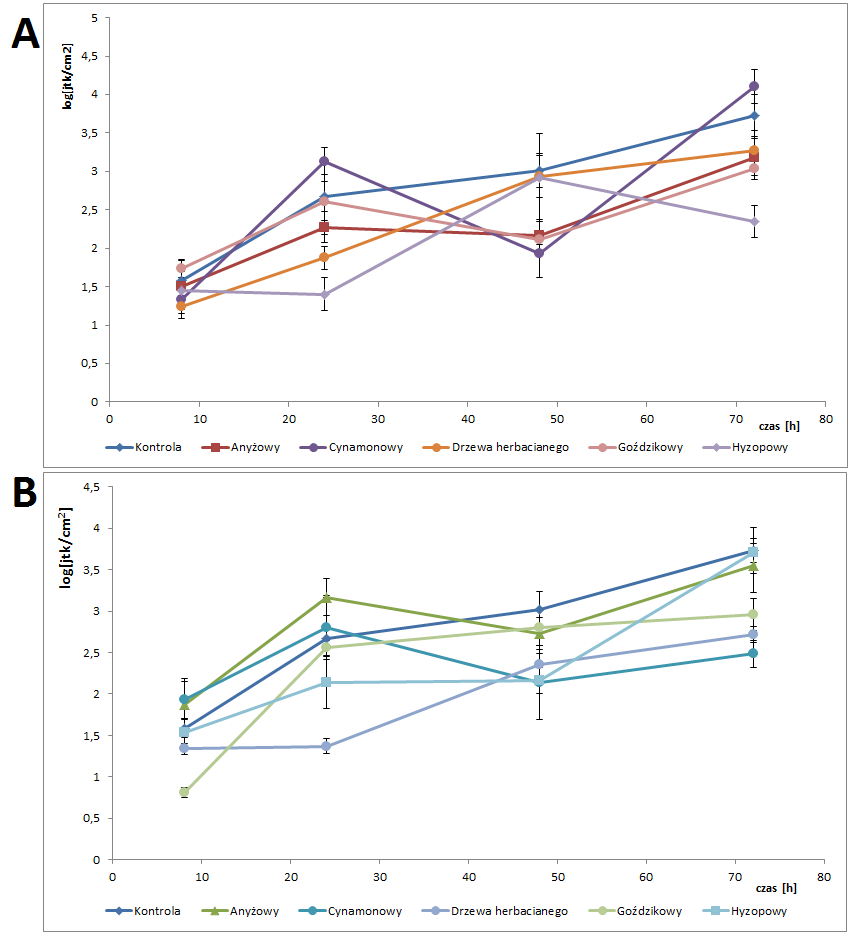
\includegraphics[scale=0.7]{img/cfii-a.png}
\caption{Dynamika tworzenia biofilmu bakterii \textit{Pseudomonas aeruginosa} CFII w obecności olejku anyżowego, cynamonowego, drzewa herbacianego, goździkowego i hyzopowego w ilości odpowiadającej A - 1/2 MIC; B - 1/4 MIC.}\label{cfii-a}
\end{center} 
\end{figure}

\begin{figure}[!h]
\begin{center}
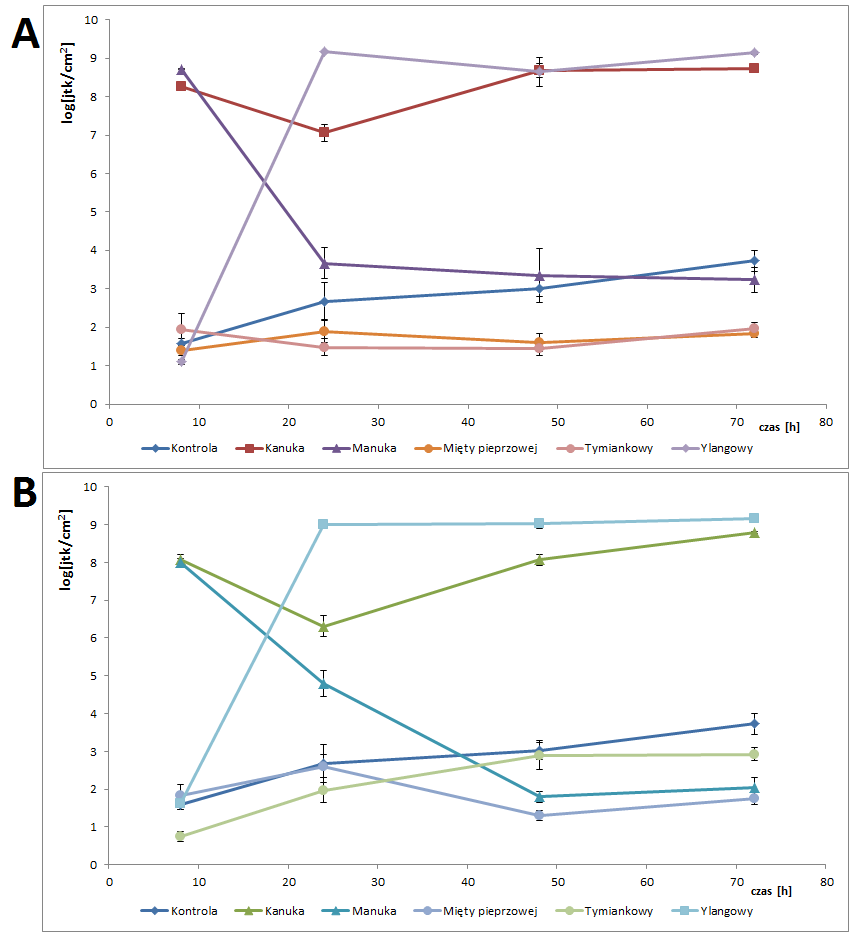
\includegraphics[scale=0.7]{img/cfii-b.png}
\caption{Dynamika tworzenia biofilmu bakterii \textit{Pseudomonas aeruginosa} CFII w obecności olejku kanuka, manuka, mięty pieprzowej, tymiankowego i ylangowego w ilości odpowiadającej A - 1/2 MIC; B - 1/4 MIC.}\label{cfii-b}
\end{center} 
\end{figure}

\clearpage

\subsection{Bakterie \textit{Pseudomonas aeruginosa} CFV}

W próbce kontrolnej biomasa biofilmu w pierwszych dwóch dobach prowadzenia hodowli przyrasta równomiernie i w 48 godzinie osiąga wartość rzędu 10$^4$jtk/cm$^2$, która utrzymuje się w trzeciej dobie hodowli. Komórki biofilmu szczepu CFV, podobnie jak w przypadku szczepu CFII, w tych samych warunkach namnażają się zdecydowanie mniejszym tempie niż komórki szczepu referencyjnego ATCC 15442.\\
W przypadku hodowli z dodatkiem olejku anyżowego, goździkowego oraz tymiankowego w stężeniach odpowiadających 1/4 wartości MIC, dynamika tworzenia się biofilmu jest zbliżona do próbki kontrolnej, co wskazywać może na znikome działanie tych dodatków na rozwój biofilmu.
Dynamika wzrostu biofilmu w hodowlach z dodatkiem olejku anyżowego i goździkowego w stężeniach odpowiadających 1/2 wartości MIC był zbliżona do próbki kontrolnej, jednak ilość biomasy w poszczególnych punktach pomiarowych była niższa o około jeden rząd wielkości.\\
Największe działanie spowalniające przyrost biomasy biofilmu zaobserwowano w przypadku hodowli z dodatkiem olejku hyzopowego w stężeniu 1/2 oraz 1/4 MIC, olejku mięty pieprzowej w stężeniu odpowiadającemu 1/4 MIC jak i z dodatkiem olejku drzewa herbacianego w stężeniach zarówno 1/2 jak i 1/4 MIC.\\
W hodowlach z dodatkiem olejku manuka oraz olejku ylangowego w obu badanych stężeniach poziom biomasy przez cały okres prowadzenia hodowli był stały i utrzymywał się na bardzo wysokim poziomie - wynosił między 8 a 9 jednostek logarytmicznych. Wartości te są zdecydowanie wyższe od ilości biomasy obserwowanej w hodowli bez dodatku olejku, co świadczyć może o pozytywnym wpływie tych dodatków na wzrost biofilmu.\\
Podobna sytuacja ma miejsce w przypadku hodowli z dodatkiem olejku kanuka. Jedynie w 8. godzinie prowadzenia hodowli poziom biomasy był niższy, dla stężenia olejku 1/2 MIC - 10$^6$jtk/cm$^2$, a dla dodatku olejku w stężeniu 1/4 - 10$^4$jtk/cm$^2$.\\
Wyższy poziom biomasy występuje także w hodowlach z dodatkiem olejku cynamonowego, gdzie w 48. godzinie prowadzenia hodowli osiąga wartości rzędu 10$^6$jtk/cm$^2$, który utrzymuje się również w trzeciej dobie.

\begin{figure}[!h]
\begin{center}
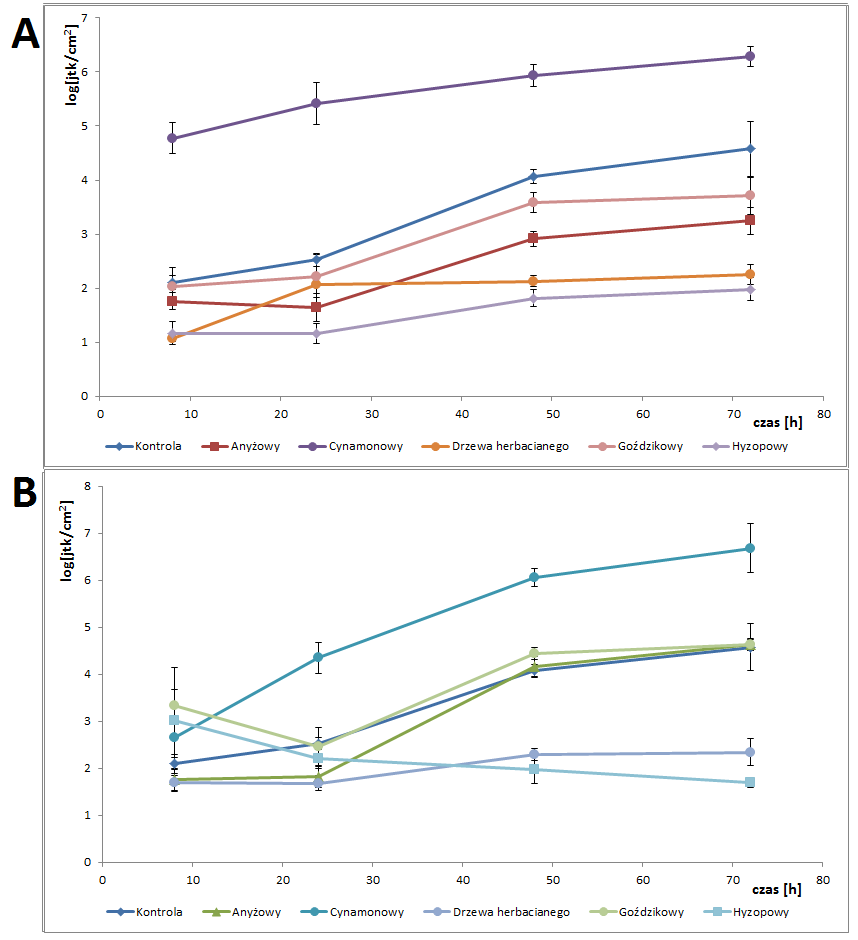
\includegraphics[scale=0.67]{img/cfv-a.png}
\caption{Dynamika tworzenia biofilmu bakterii \textit{Pseudomonas aeruginosa} CFV w obecności olejku anyżowego, cynamonowego, drzewa herbacianego, goździkowego i hyzopowego w ilości odpowiadającej A - 1/2 MIC; B - 1/4 MIC.}\label{cfv-a}
\end{center} 
\end{figure}

\begin{figure}[!h]
\begin{center}
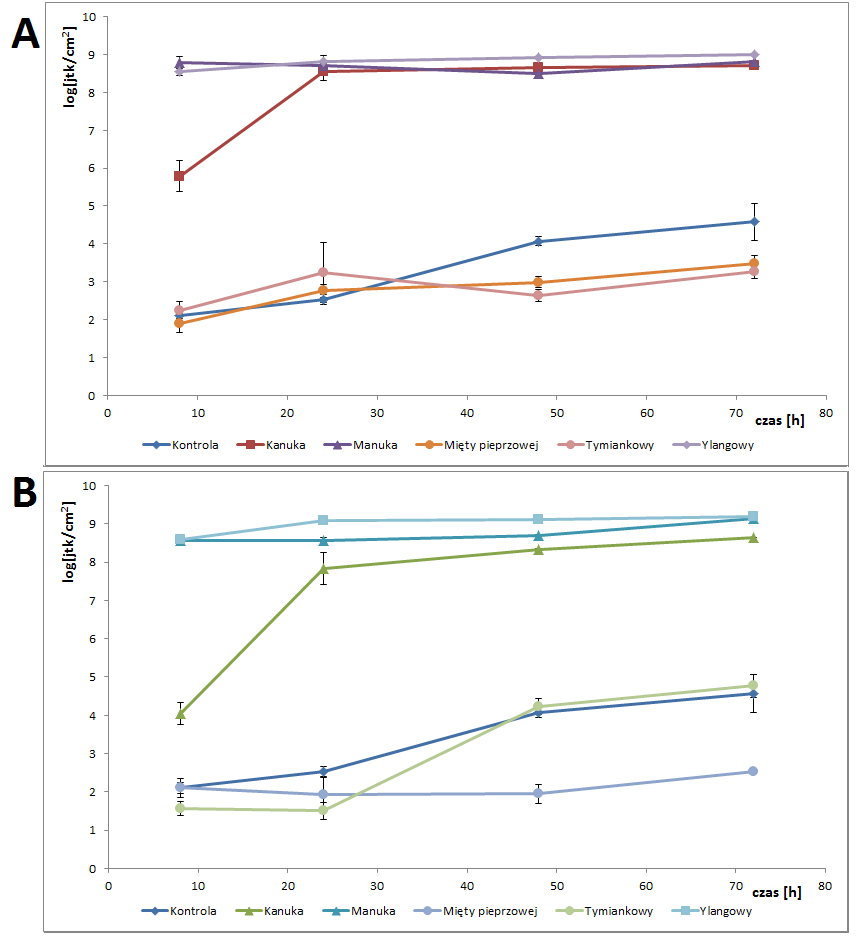
\includegraphics[scale=0.7]{img/cfv-b.png}
\caption{Dynamika tworzenia biofilmu bakterii \textit{Pseudomonas aeruginosa} CFV w obecności olejku kanuka, manuka, mięty pieprzowej, tymiankowego i ylangowego w ilości odpowiadającej A - 1/2 MIC; B - 1/4 MIC.}\label{cfv-b}
\end{center} 
\end{figure}

\clearpage


\subsection{Bakterie \textit{Pseudomonas cedrina} PC}

W pierwszych dwóch dobach prowadzenia hodowli biomasa w próbce kontrolnej przyrasta równomiernie i w 48 godzinie osiąga wartość rzędu 10$^7$jtk/cm$^2$, która utrzymuje się w trzeciej dobie hodowli.\\
Dynamika wzrostu biofilmu w hodowlach z dodatkiem olejku manuka w stężeniu odpowiadającym 1/2 wartości MIC była bardzo podobna do dynamiki obserwowanej dla próbki kontrolnej. Podobnymi do kontroli wartościami w 24., 48. i 72. godzinie charakteryzują się hodowle z dodatkiem olejku anyżowego w stężeniu 1/4 MIC oraz olejku drzewa herbacianego w obu stężeniach, jednak w 8. godzinie ilość biomasy jest znacznie niższa niż dla próbki kontrolnej.
Te dodatki do hodowli nie wpływają w sposób znaczący na rozwój tego biofilmu bakteryjnego.\\
Dla próbek z dodatkiem olejku anyżowego w stężeniu odpowiadającemu 1/2 wartości MIC, olejku cynamonowego (1/4 MIC), goździkowego (1/2 MIC), hyzopowego (1/4 MIC) oraz olejku manuka (1/4 MIC) dynamika wzrostu biofilmu jest zbliżona do próbki kontrolnej, jednak ilość biomasy w poszczególnych punktach pomiarowych była niższa o około jeden rząd wielkości.\\
W przypadku hodowli z dodatkiem olejku mięty pieprzowej w obu badanych stężeniach a także w obecności olejku tymiankowego (1/2 MIC) zaobserwowano najsilniejsze działanie spowalniające rozrost biofilmu - w trzeciej dobie hodowli ilość biomasy nie przekraczała 5 jednostek logarytmicznych.\\
Charakterystyczną dynamiką wzrostu biofilmu odznaczały się próbki z dodatkiem olejku goździkowego w stężeniu odpowiadającemu 1/4 MIC, olejku hyzopowego (1/2 MIC), olejku kanuka (w obu badanych stężeniach) oraz olejku tymiankowego w stężeniu 1/4 MIC. W 8. i 24. godzinie prowadzenia hodowli liczba komórek biofilmu jest niska - oscyluje w granicach 1-2 jednostek logarytmicznych. W drugiej i trzeciej dobie wartości te intensywnie wzrastają i osiągają poziom próbki kontrolnej. Dynamika wzrostu tych hodowli może świadczyć o tym, iż dodatki te działają hamująco na rozwój biofilmu jedynie przy krótkim czasie kontaktu.\\
Dodatek olejku ylangowego stymuluje rozwój badanego biofilmu. Jego poziom już w 8. godzinie, dla obu badanych stężeń, był rzędu 8,5-9 jednostek logarytmicznych i utrzymywał się przez cały czas prowadzenia hodowli.

\begin{figure}[!h]
\begin{center}
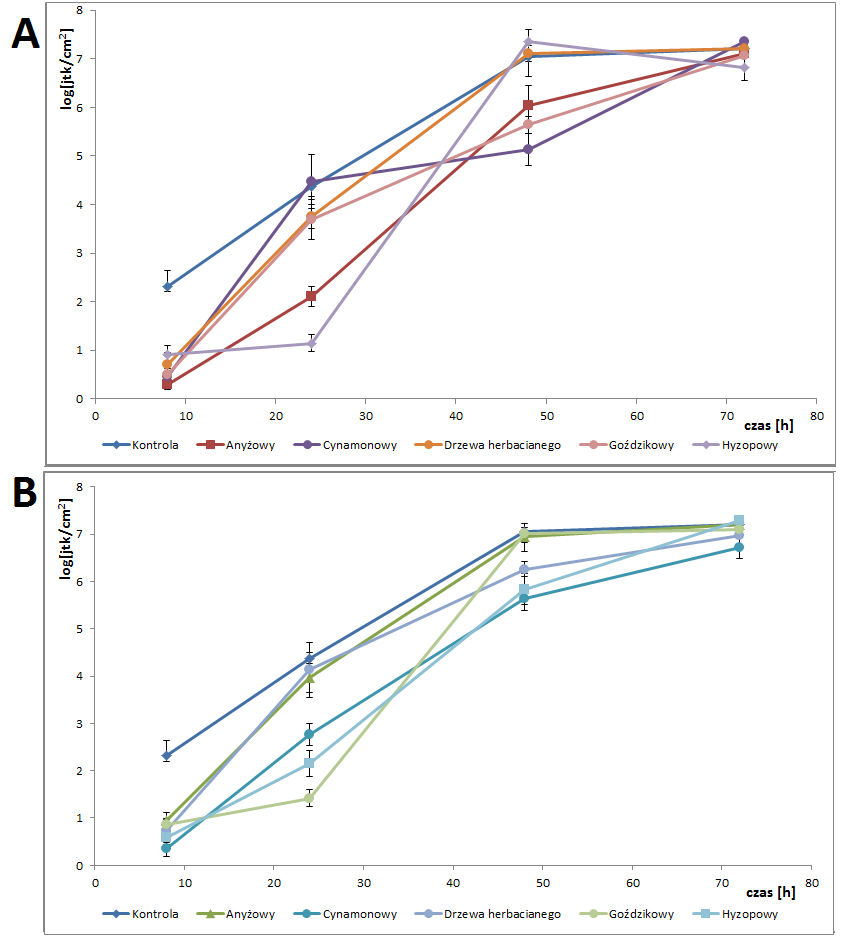
\includegraphics[scale=0.61]{img/pc-a.png}
\caption{Dynamika tworzenia biofilmu bakterii \textit{Pseudomonas cedrina} DH1 w obecności olejku anyżowego, cynamonowego, drzewa herbacianego, goździkowego i hyzopowego w ilości odpowiadającej A - 1/2 MIC; B - 1/4 MIC.}\label{pc-a}
\end{center} 
\end{figure}

\begin{figure}[!h]
\begin{center}
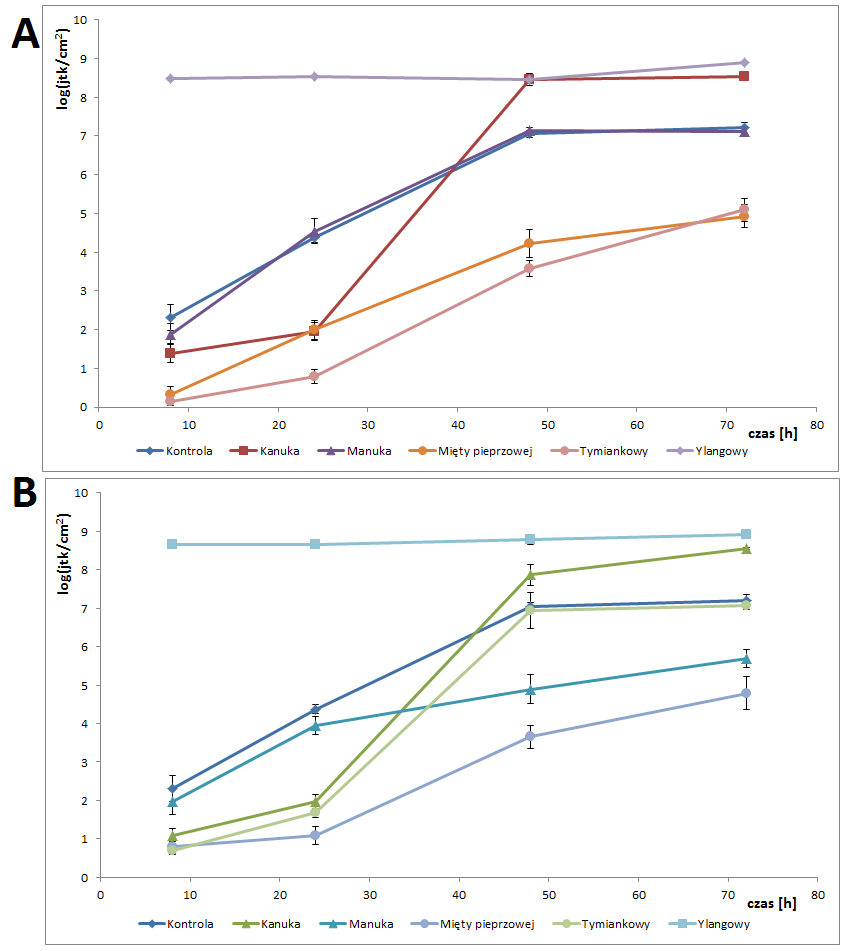
\includegraphics[scale=0.7]{img/pc-b.png}
\caption{Dynamika tworzenia biofilmu bakterii \textit{Pseudomonas cedrina} DH1 w obecności olejku kanuka, manuka, mięty pieprzowej, tymiankowego i ylangowego w ilości odpowiadającej A - 1/2 MIC; B - 1/4 MIC.}\label{pc-b}
\end{center} 
\end{figure}

\clearpage

\subsection{Bakterie \textit{Pseudomonas cedrina} DH1}

W pierwszej dobie prowadzenia hodowli biomasa w próbce kontrolnej utrzymuje się na niskim poziomie - przyrasta od 1,5 w 8. godzinie do 2 jednostek logarytmicznych po 24 godzinach. W 48. godzinie osiąga wartość rzędu 10$^7$jtk/cm$^2$, która wzrasta w trzeciej dobie hodowli do wartości rzędu 10$^8$jtk/cm$^2$. Wartości bardzo zbliżone do tych, uzyskanych w próbce kontrolnej wykazują hodowle z dodatkiem olejku cynamonowego w obu badanych stężeniach. Wynika z tego, iż olejek ten nie wpływa w znaczący sposób na rozwój biofilmu bakterii \textit{Pseudomonas cedrina} DH1.\\
Najsilniejsze działanie hamujące przyrost biofilmu zaobserwowano w hodowlach z dodatkiem olejku anyżowego w stężeniu odpowiadającemu 1/2 wartości MIC, olejku drzewa herbacianego w obu badanych stężeniach, olejku goździkowego (1/2 MIC) oraz olejku mięty pieprzowej w obu stężeniach. Najbardziej znaczące różnice między tymi hodowlami a próbką kontrolną widoczne są w drugiej i trzeciej dobie, gdzie poziom biomasy jest co najmniej o jeden rząd wielkości mniejszy.\\
W hodowlach z dodatkiem olejku anyżowego dodanym w stężeniu 1/4 wartości MIC, olejku goździkowego (1/4 MIC), olejku hyzopowego oraz tymiankowego w obydwu badanych stężeniach dynamika wzrostu jest zbliżona do próbki kontrolnej, jednak wyraźna różnica obserwowana jest w 48. godzinie, gdzie ilość biomasy w hodowlach z dodatkiem olejków jest zdecydowanie niższa - o co najmniej 2 rzędy wielkości.Olejki te w bardzo niewielkim stopniu wpływają na hamowanie rozwoju biofilmu, przy dłuższym kontakcie poziom biomasy w tych próbkach nie odbiega znacząco od kontroli.\\
Dla próbek z dodatkiem olejku kanuka oraz manuka w stężeniu 1/4 MIC oraz olejku ylangowego (1/2 MIC) w 8. godzinie hodowli ilość biomasy w nie odbiegała znacząco od wartości dla próbki kontrolnej. W 24. godzinie wartości te wzrastają do poziomu o co najmniej 2 jednostki logarytmiczne wyższego od tych dla próbki kontrolnej. W kolejnych dobach ilość biomasy w hodowlach z dodatkiem olejków wzrasta niemal liniowo i w trzeciej dobie osiąga wartości zbliżone do próbki olejków. Obecność tych olejków w pierwszej dobie hodowli przyspiesza rozwój biofilmu, jednak przy wydłużonym kontakcie nie wpływa znacząco na jego poziom.

\begin{figure}[!h]
\begin{center}
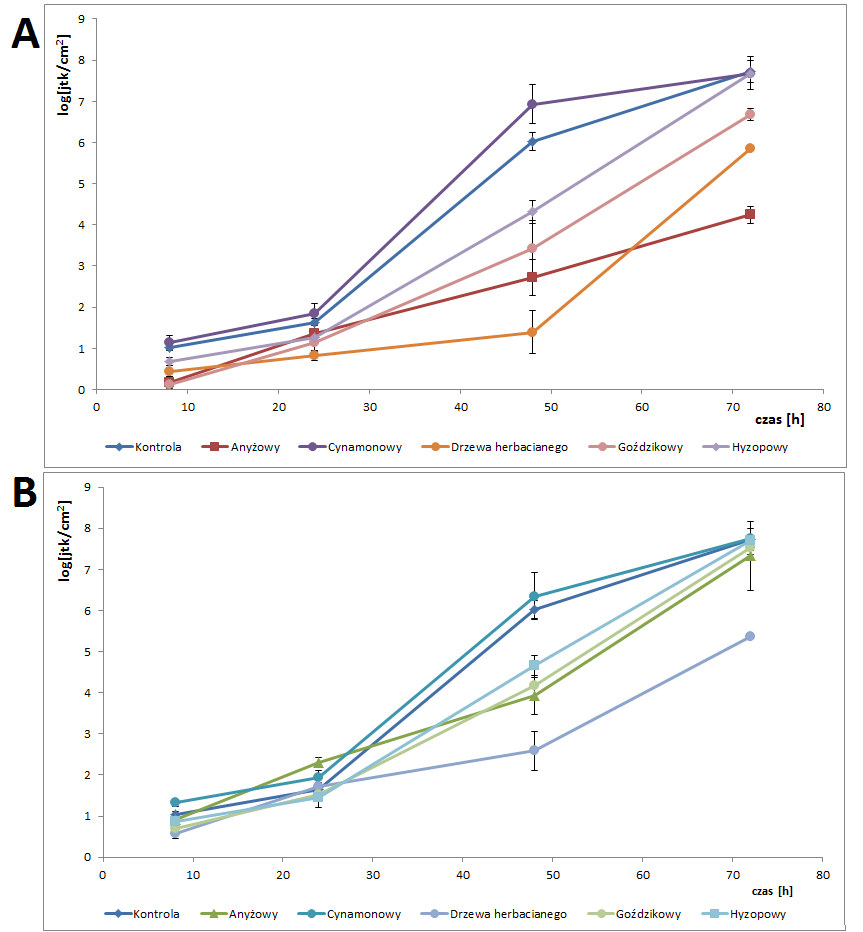
\includegraphics[scale=0.68]{img/dh1-a.png}
\caption{Dynamika tworzenia biofilmu bakterii \textit{Pseudomonas cedrina} DH1 w obecności olejku anyżowego, cynamonowego, drzewa herbacianego, goździkowego i hyzopowego w ilości odpowiadającej A - 1/2 MIC; B - 1/4 MIC.}\label{dh1-a}
\end{center} 
\end{figure}

\begin{figure}[!h]
\begin{center}
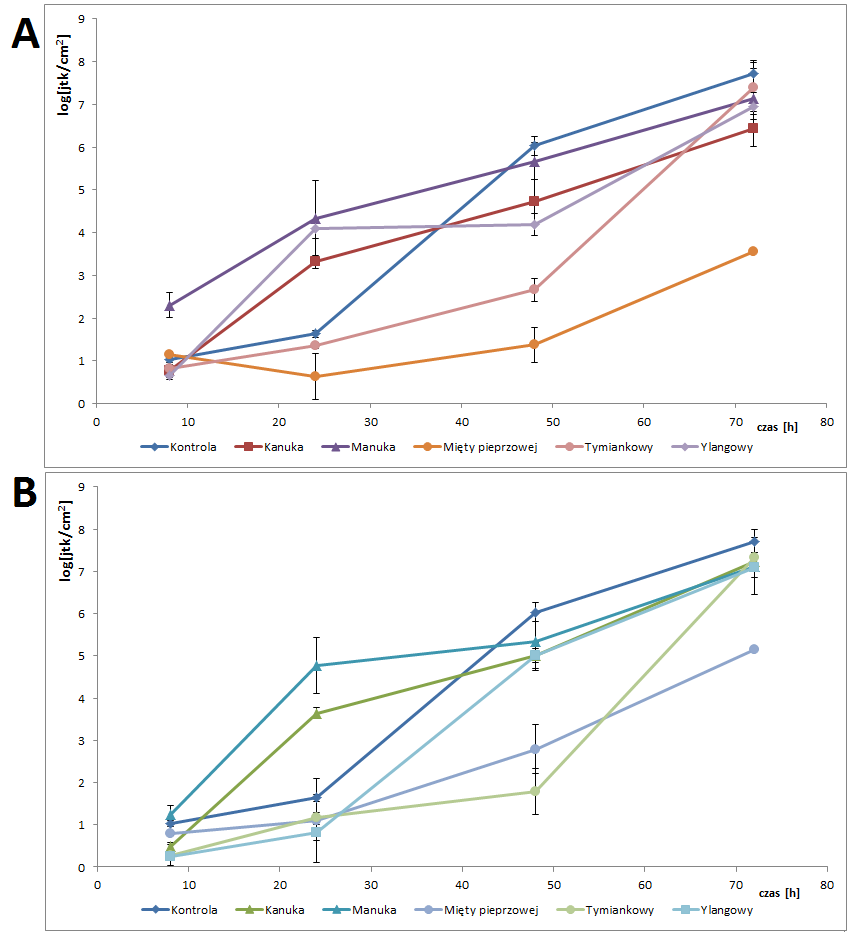
\includegraphics[scale=0.7]{img/dh1-b.png}
\caption{Dynamika tworzenia biofilmu bakterii \textit{Pseudomonas cedrina} DH1 w obecności olejku kanuka, manuka, mięty pieprzowej, tymiankowego i ylangowego w ilości odpowiadającej A - 1/2 MIC; B - 1/4 MIC.}\label{dh1-b}
\end{center} 
\end{figure}

\clearpage

\subsection{Bakterie \textit{Pseudomonas cedrina} DH2}

W próbce kontrolnej biomasa biofilmu w pierwszych dwóch dobach prowadzenia hodowli przyrasta równomiernie i w 48 godzinie osiąga wartość rzędu 10$^8$jtk/cm$^2$; poziom ten utrzymuje się w trzeciej dobie hodowli.\\
Hodowle z dodatkiem olejku anyżowego i goździkowego w stężeniu 1/4 MIC charakteryzują się podobną dynamiką wzrostu do próby kontrolnej. Nieznaczne różnice w ilości biomasy występują jedynie w 24. godzinie prowadzenia hodowli.\\
Zdecydowanie najsilniejszym działaniem hamującym rozwój biofilmu odznacza się dodatek olejku mięty pieprzowej w stężeniu odpowiadającym 1/2 wartości MIC - w ciągu pierwszych 48. godzin prowadzenia hodowli ilość biomasy jest bardzo niska, nie przekracza 5 jtk/cm$^2$. Dopiero w trzeciej dobie prowadzenia hodowli wartość ta wzrasta do poziomu 3,5 jednostek logarytmicznych.\\
W hodowli z dodatkiem olejku hyzopowego w stężeniu odpowiadającemu 1/2 wartości MIC również zaobserwowano silne działanie hamujące rozwój biofilmu - poziom ilości biomasy przez cały okres trwania hodowli nie przekraczał 2 jednostek logarytmicznych. W podobnym stopniu hamująco na wzrost biomasy działał dodatek olejku drzewa herbacianego w stężeniu 1/4 MIC - ilość biomasy wzrastała równomiernie i powoli, w trzeciej dobie osiągając wartość 3,5 jednostek logarytmicznych.\\
Działanie hamujące  wzrost biofilmu przy wydłużonym czasie kontaktu wykazują dodatki olejku kanuka oraz manuka w obu badanych stężeniach oraz olejku ylangowego i olejku mięty pieprzowej w stężeniach odpowiadających 1/4 wartości MIC. W ciągu pierwszej doby ilość biomasy w tych próbkach wzrasta podobnie do hodowli kontrolnej, po czym stabilizuje się, osiągając wartości rzędu 10$^3$-10$^5$jtk/cm$^2$.\\
Dodatek olejku cynamonowego (w obu stężeniach), hyzopowego w stężeniu odpowiadającym 1/4 wartości MIC oraz olejku tymiankowego (1/2 MIC) do hodowli działa hamująco na wzrost biofilmu zwłaszcza w ciągu pierwszych 48 godzin. Ilość biomasy w tych próbkach wzrasta niemal liniowo, jednak w trzeciej dobie następuje wyraźny przyrost biofilmu, którego ilość w 72. godzinie zbliża się do wartości próbki kontrolnej.

\begin{figure}[!h]
\begin{center}
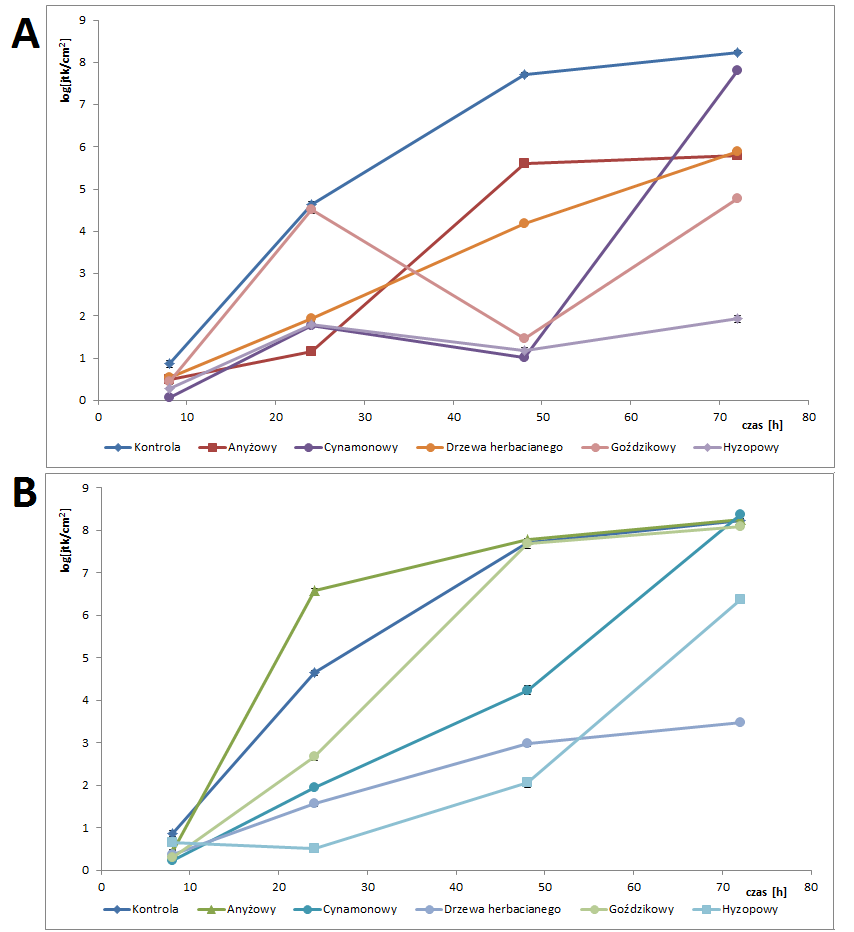
\includegraphics[scale=0.68]{img/dh2-a.png}
\caption{Dynamika tworzenia biofilmu bakterii \textit{Pseudomonas cedrina} DH1 w obecności olejku anyżowego, cynamonowego, drzewa herbacianego, goździkowego i hyzopowego w ilości odpowiadającej A - 1/2 MIC; B - 1/4 MIC.}\label{dh2-a}
\end{center} 
\end{figure}

\begin{figure}[!h]
\begin{center}
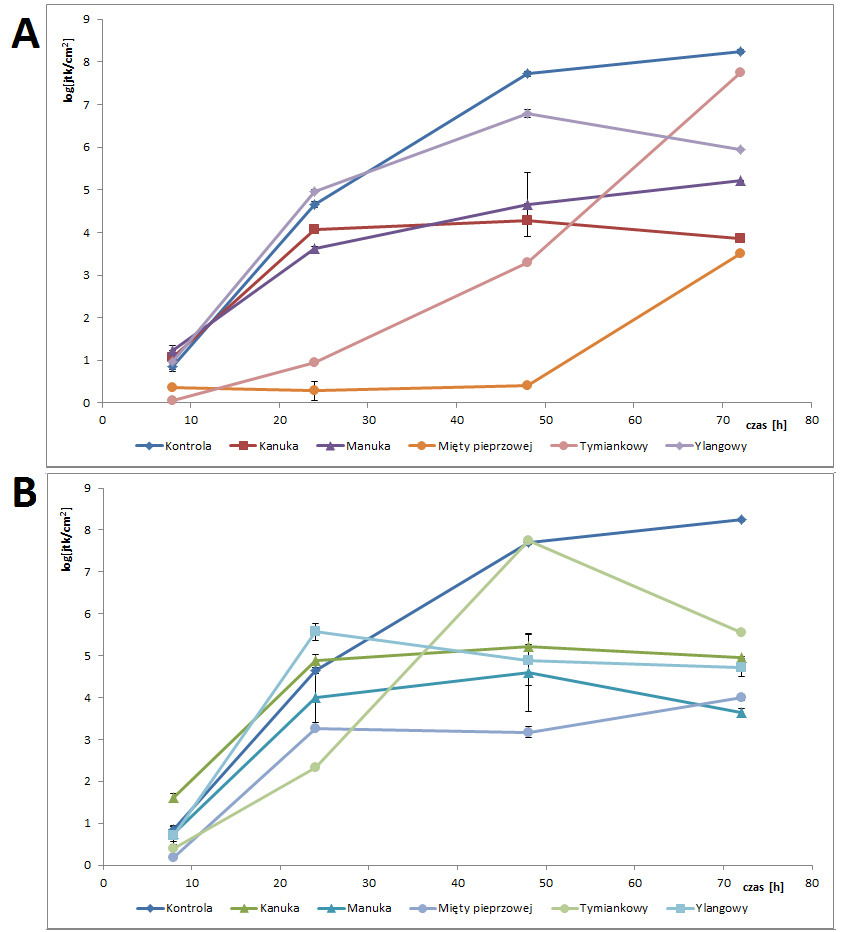
\includegraphics[scale=0.7]{img/dh2-b.png}
\caption{Dynamika tworzenia biofilmu bakterii \textit{Pseudomonas cedrina} DH1 w obecności olejku kanuka, manuka, mięty pieprzowej, tymiankowego i ylangowego w ilości odpowiadającej A - 1/2 MIC; B - 1/4 MIC.}\label{dh2-b}
\end{center} 
\end{figure}

\clearpage

\section{Dynamika wzrostu bakterii w formie planktonu w obecności olejków eterycznych}

%\subsection{Bakterie \textit{Pseudomonas aeruginosa} ATCC 15442}
Dla szczepu \textit{Pseudomonas cedrina} ATCC 15442 w próbce bez dodatku olejku liczba komórek planktonu w 8. godzinie hodowli była rzędu 10$^5$jtk/cm$^3$, w 24. godzinie wzrosła do poziomu 10$^10$jtk/cm$^3$. Poziom ten utrzymał się do końca prowadzenia hodowli.\\
Dynamika wzrostu biomasy planktonu w hodowlach z dodatkiem olejków eterycznych, z wyjątkiem tych z olejkiem mięty pieprzowej, nie odbiegała znacząco od próbki kontrolnej. Niewielkie różnice zaobserwowano w 8. godzinie prowadzenia hodowli - dla próbki z dodatkiem olejku anyżowego ilość komórek planktonu była wyższa o 2 rzędy wielkości i wynosiła 7,5 jednostek logarytmicznych, zaś poziom ilości planktonu w próbkach z dodatkiem pozostałych olejków był niższy od wartości dla próbki kontrolnej i oscylowały w granicach rzędu 10$^2$-10$^5$jtk/cm$^3$. Dodatki tych olejków mają znikomy wpływ na rozwój planktonu.\\
Wyjątek stanowiła próbka z dodatkiem olejku mięty pieprzowej. W 8. godzinie prowadzenia hodowli ilość biomasy planktonu była znikoma - nie przekraczała 10jtk/cm$^3$. Liczba komórek planktonu rosła liniowo w drugiej dobie osiągając wartość zbliżoną do próby kontrolnej rzędu 10$^9$jtk/cm$^3$, która utrzymuje się do końca prowadzenia hodowli. Świadczy to o dość silnym działaniu hamującym rozwój biofilmu, które zanika wraz z wydłużaniem czasu kontaktu.

\begin{figure}[!h]
\begin{center}
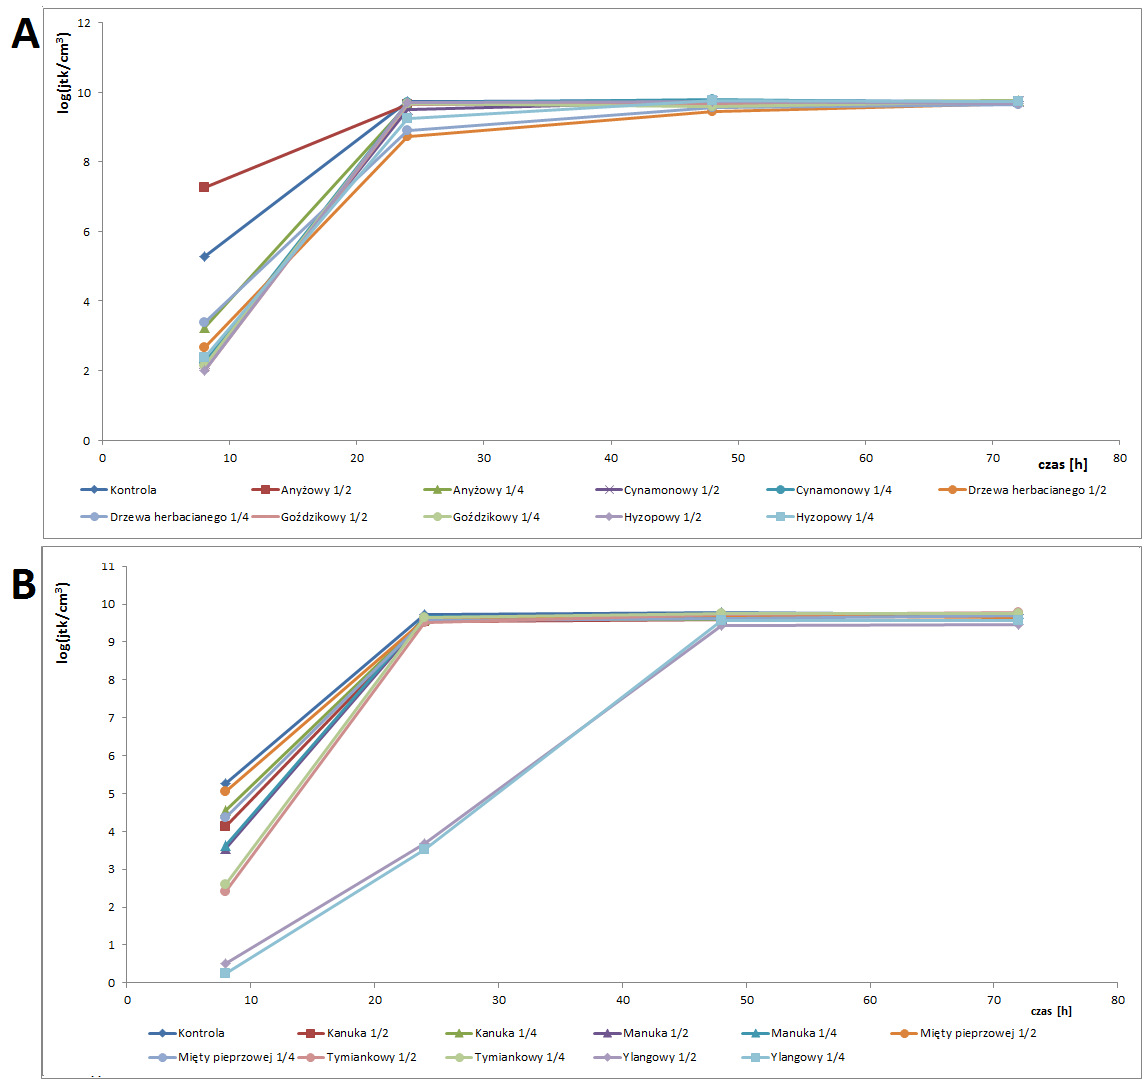
\includegraphics[scale=0.50]{img/ref-c.png}
\caption{Dynamika tworzenia biofilmu bakterii \textit{Pseudomonas cedrina} ATCC 15442 w obecności olejków w stężeniu odpowiadającemu 1/2 oraz 1/4 MIC; A - olejek anyżowy, cynamonowy, drzewa herbacianego, goździkowy i hyzopowy, B - olejek kanuka, manuka, mięty pieprzowej, tymiankowy i ylangowy.}\label{ref-c}
\end{center} 
\end{figure}

\clearpage

%\subsection{Bakterie \textit{Pseudomonas aeruginosa} CFII}
Dynamika wzrostu dla planktonu bakterii szczepu CFII była odmienna niż dla szczepu ATCC 15442. Ilość komórek dla próby kontrolnej w pierwszej dobie prowadzenia hodowli nieznacznie wzrosła z 9,3 do 9,6 jednostek logarytmicznych, po czym ustabilizowała się na tym poziomie.\\
W hodowlach z dodatkiem olejków dynamika wzrostu była bardzo zbliżona, a uzyskiwane wartości oscylowały w granicach 8,6-9,7 jednostek logarytmicznych.

\begin{figure}[!h]
\begin{center}
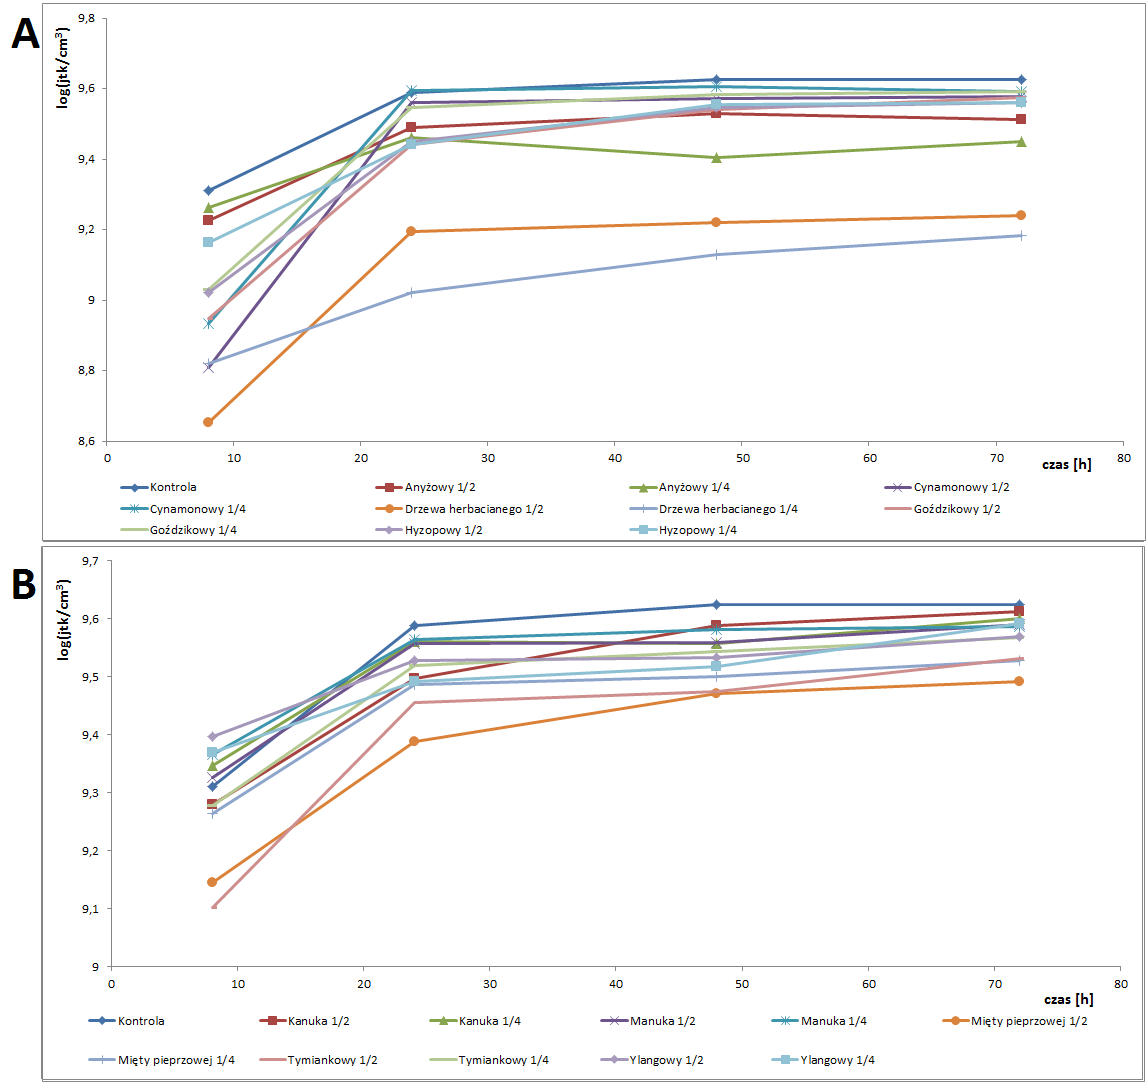
\includegraphics[scale=0.50]{img/cfii-c.png}
\caption{Dynamika tworzenia biofilmu bakterii \textit{Pseudomonas cedrina} CFII w obecności olejków w stężeniu odpowiadającemu 1/2 oraz 1/4 MIC; A - olejek anyżowy, cynamonowy, drzewa herbacianego, goździkowy i hyzopowy, B - olejek kanuka, manuka, mięty pieprzowej, tymiankowy i ylangowy.}\label{cfii-c}
\end{center} 
\end{figure}

\clearpage

%\subsection{Bakterie \textit{Pseudomonas aeruginosa} CFV}
Dynamika wzrostu hodowli szczepu \textit{Pseudomonas cedrina} CFV była podobna do dynamiki szczepu CFII. Liczba komórek planktonu w próbce kontrolnej przez cały okres prowadzenia hodowli była na poziomie 10$^10$jtk/cm$^3$.\\
Dla hodowli z dodatkiem olejków, poza olejkiem drzewa herbacianego ilość biomasy kształtowała się w granicach 10$^9$-10$^10$jtk/cm$^3$, co świadczy o znikomym wpływie tych dodatków na rozwój planktonu.\\
Wyjątek stanowiła próbka z dodatkiem olejku drzewa herbacianego w stężeniu odpowiadającemu 1/2 wartości MIC; w 8. godzinie hodowli liczba komórek wynosiła 10$^5$jtk/cm$^3$, zaś po 24 godzinach - 10$^8$jtk/cm$^3$. Wskazuje to na działanie hamujące olejku drzewa herbacianego, które jednak zanika przy wydłużonym czasie kontaktu.

\begin{figure}[!h]
\begin{center}
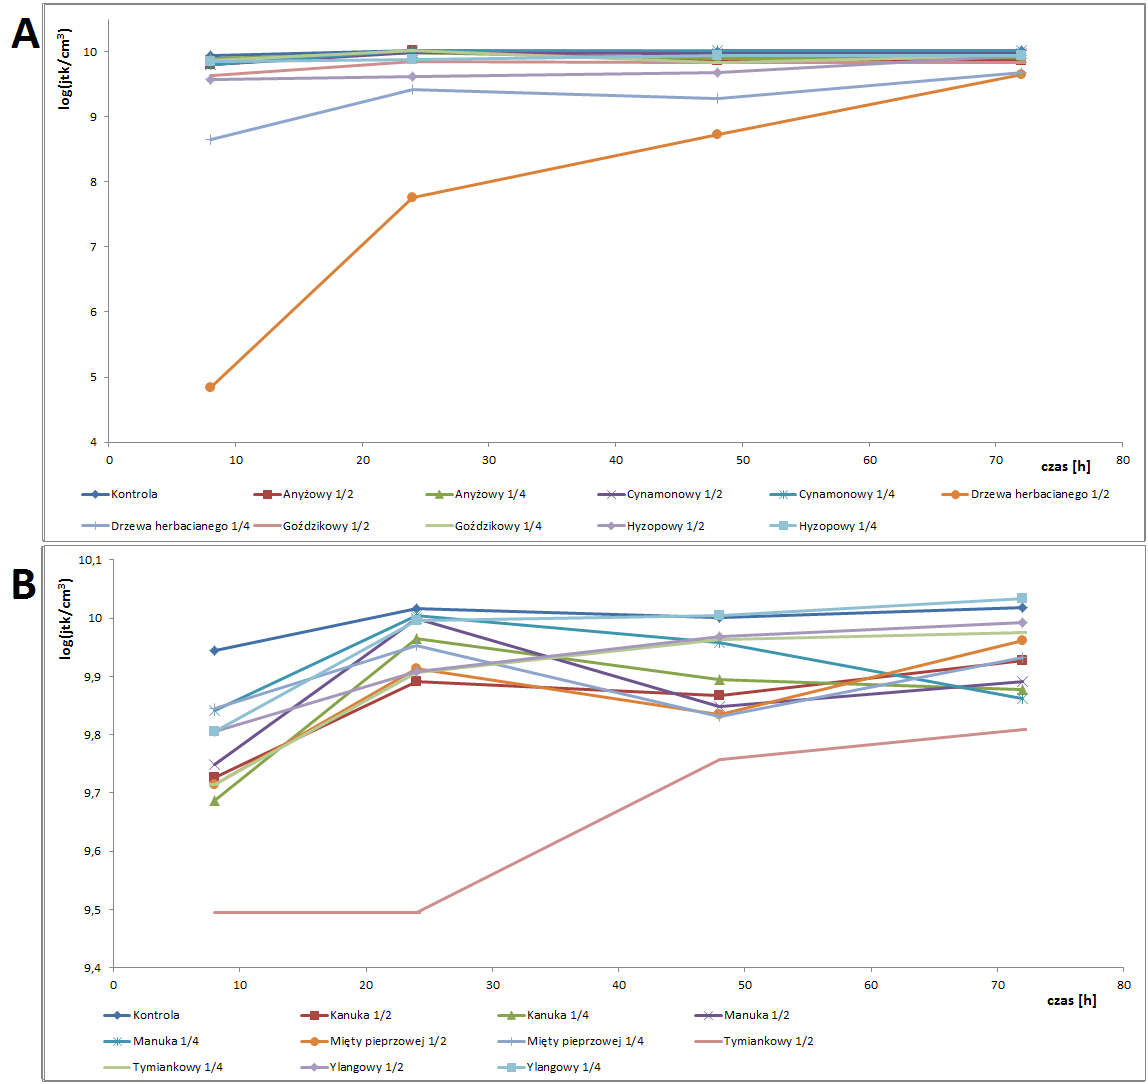
\includegraphics[scale=0.50]{img/cfv-c.png}
\caption{Dynamika tworzenia biofilmu bakterii \textit{Pseudomonas cedrina} CFV w obecności olejków w stężeniu odpowiadającemu 1/2 oraz 1/4 MIC; A - olejek anyżowy, cynamonowy, drzewa herbacianego, goździkowy i hyzopowy, B - olejek kanuka, manuka, mięty pieprzowej, tymiankowy i ylangowy.}\label{cfv-c}
\end{center} 
\end{figure}

\clearpage

%\subsection{Bakterie \textit{Pseudomonas cedrina} PC}
Podobnie jak w przypadku szczepu \textit{Pseudomonas aeruginosa} CFV, wobec bakterii planktonowych szczepu \textit{Pseudomonas cedrina} PC jedynie stężenie 1/2 MIC olejku drzewa herbacianego w znaczący sposób wpływa na dynamikę wzrostu komórek planktonowych. Pozostałe hodowle, tak jak kontrola, nieznacznie wzrastają i oscylują w granicach 8,4-9,5 jednostek logarytmicznych. Swiadczy to o braku znaczącego wpływu na ilość biomasy planktonu w hodowli.\\
Dla próbki z dodatkiem olejku drzewa herbacianego w stężeniu 1/2 MIC wartości uzyskiwane w pierwszej dobie hodowli są zdecydowanie niższe od wartości dla próby kontrolnej; w 8. godzinie - 2, zaś w 24. godzinie - 4,5 jednostek logarytmicznych. Wskazuje to na działanie hamujące tego olejku na wzrost planktonu tych bakterii. Zanika ono jednak wraz z wydłużaniem czasu kontaktu.

\begin{figure}[!h]
\begin{center}
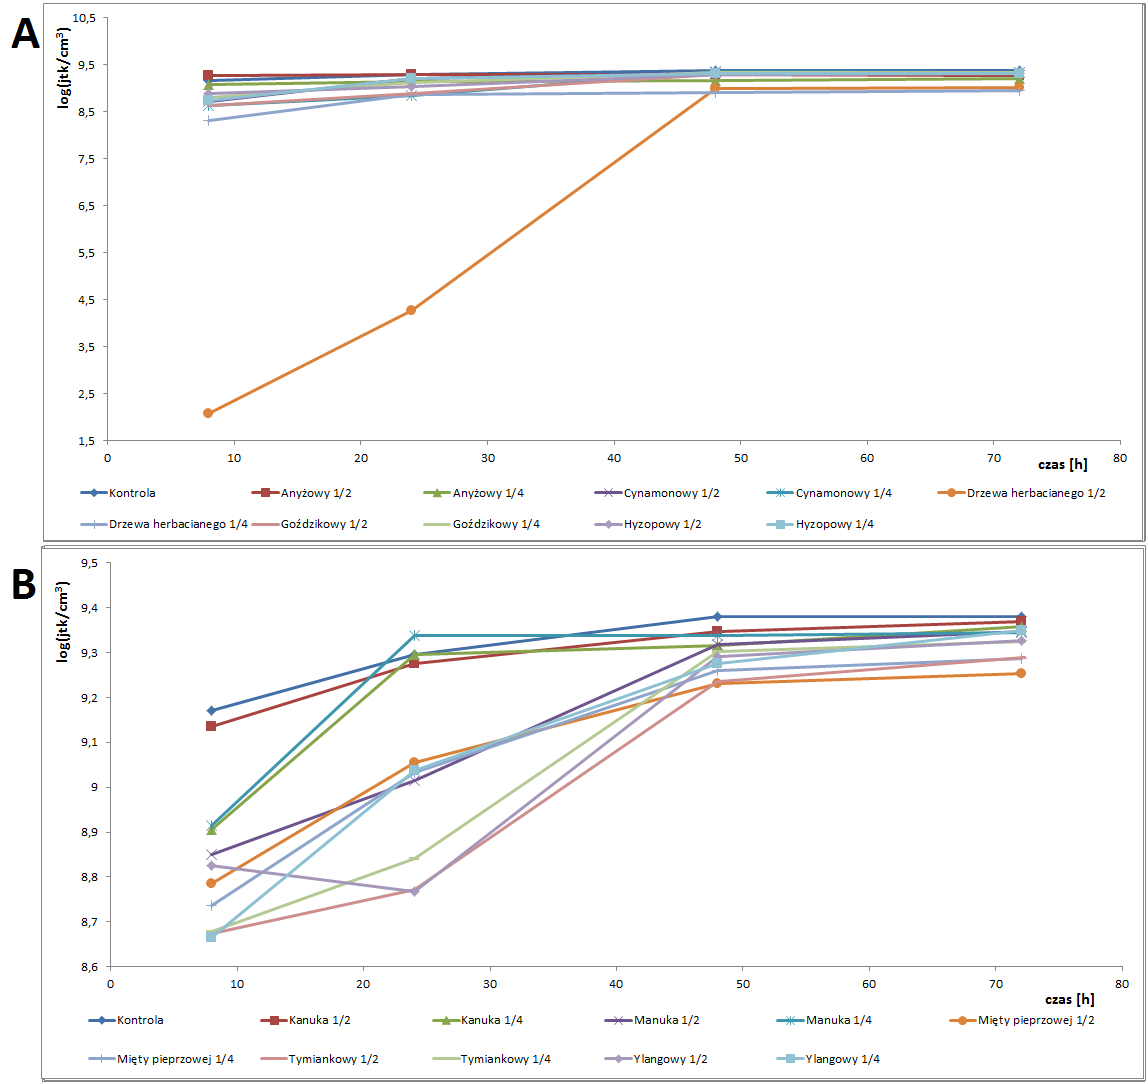
\includegraphics[scale=0.55]{img/pc-c.png}
\caption{Dynamika tworzenia biofilmu bakterii \textit{Pseudomonas cedrina} PC w obecności olejków w stężeniu odpowiadającemu 1/2 oraz 1/4 MIC; A - olejek anyżowy, cynamonowy, drzewa herbacianego, goździkowy i hyzopowy, B - olejek kanuka, manuka, mięty pieprzowej, tymiankowy i ylangowy.}\label{pc-c}
\end{center} 
\end{figure}

\clearpage

%\subsection{Bakterie \textit{Pseudomonas cedrina} DH1}

Dla próbki kontrolnej szczepu \textit{Pseudomonas cedrina} DH1 dynamika wzrostu komórek planktonowych kształtuje się podobnie do szczepu PC. W 8. godzinie hodowli ilość komórek wynosi 10$^9$jtk/cm$^3$, po czym nieznacznie wzrasta i po 48 godzinach stabilizuje się na poziome 9,3 jednostek logarytmicznych.\\
Dynamika wzrostu wszystkich hodowli z dodatkami olejków jest zbliżona do próbki kontrolnej i oscyluje w granicach 10$^8$-10$^10$jtk/cm$^3$. dodatki badanych olejków eterycznych nie wpływają w znaczący sposób na ilość komórek planktonu w hodowli szczepu DH1.

\begin{figure}[!h]
\begin{center}
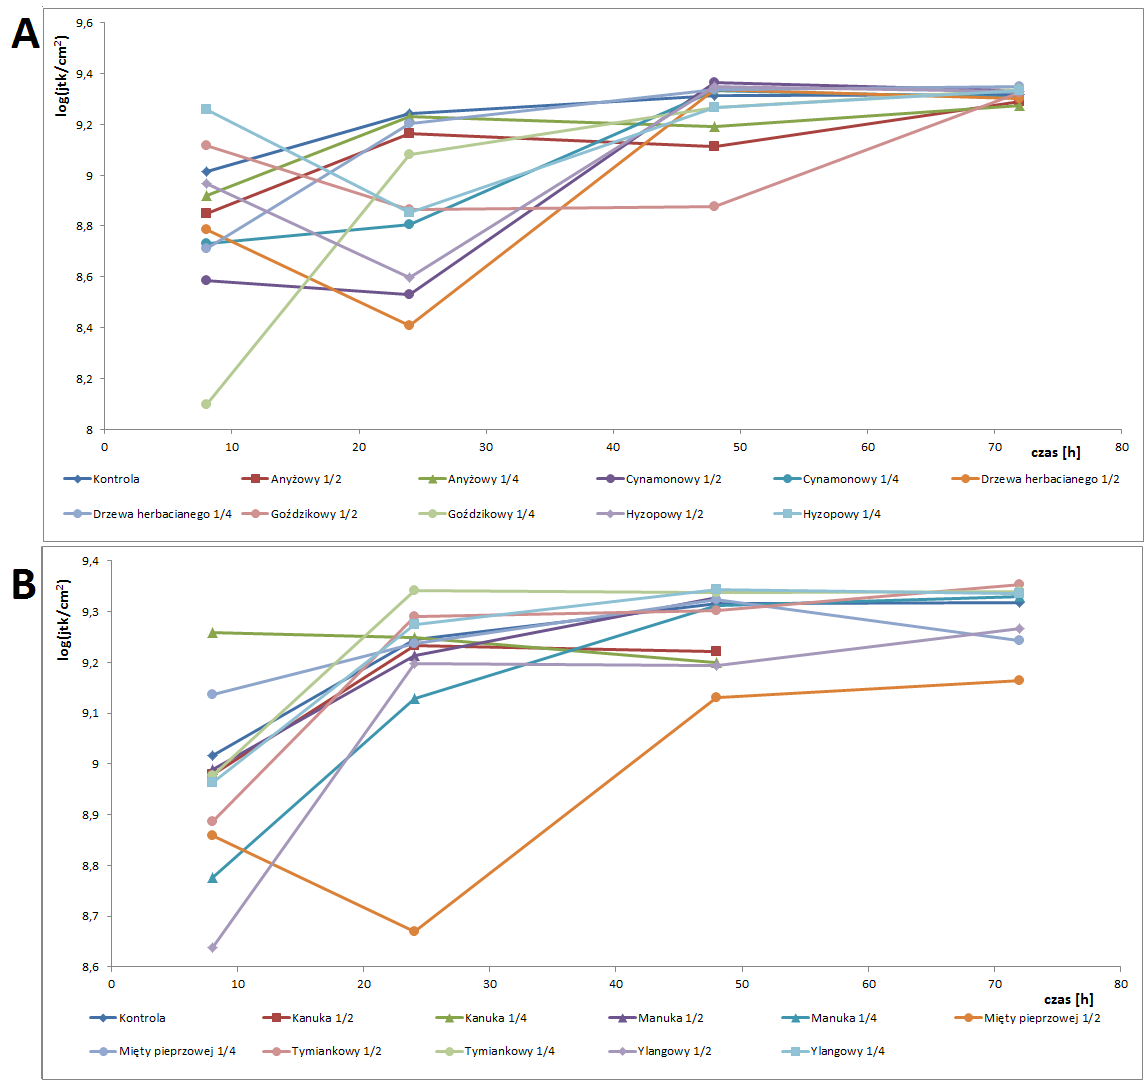
\includegraphics[scale=0.55]{img/dh1-c.png}
\caption{Dynamika tworzenia biofilmu bakterii \textit{Pseudomonas cedrina} DH1 w obecności olejków w stężeniu odpowiadającemu 1/2 oraz 1/4 MIC; A - olejek anyżowy, cynamonowy, drzewa herbacianego, goździkowy i hyzopowy, B - olejek kanuka, manuka, mięty pieprzowej, tymiankowy i ylangowy.}\label{dh1-c}
\end{center} 
\end{figure}

\clearpage

%\subsection{Bakterie \textit{Pseudomonas cedrina} DH2}

Dynamika wzrostu ilości biomasy w próbce kontrolnej jest bardzo zbliżona do pozostałych \textit{Pseudomonas cedrina} i kształtuje się na poziomie 8,5-8,9 jednostek logarytmicznych.\\
Wartości dla hodowli z dodatkiem olejków eterycznych są nieznacznie niższe i oscylują w granicach 8,2-8,9 jednostek logarytmicznych. Żaden z badanych dodatków nie wpływa w sposób znaczący na ilość wytworzonej biomasy planktonu.

\begin{figure}[!h]
\begin{center}
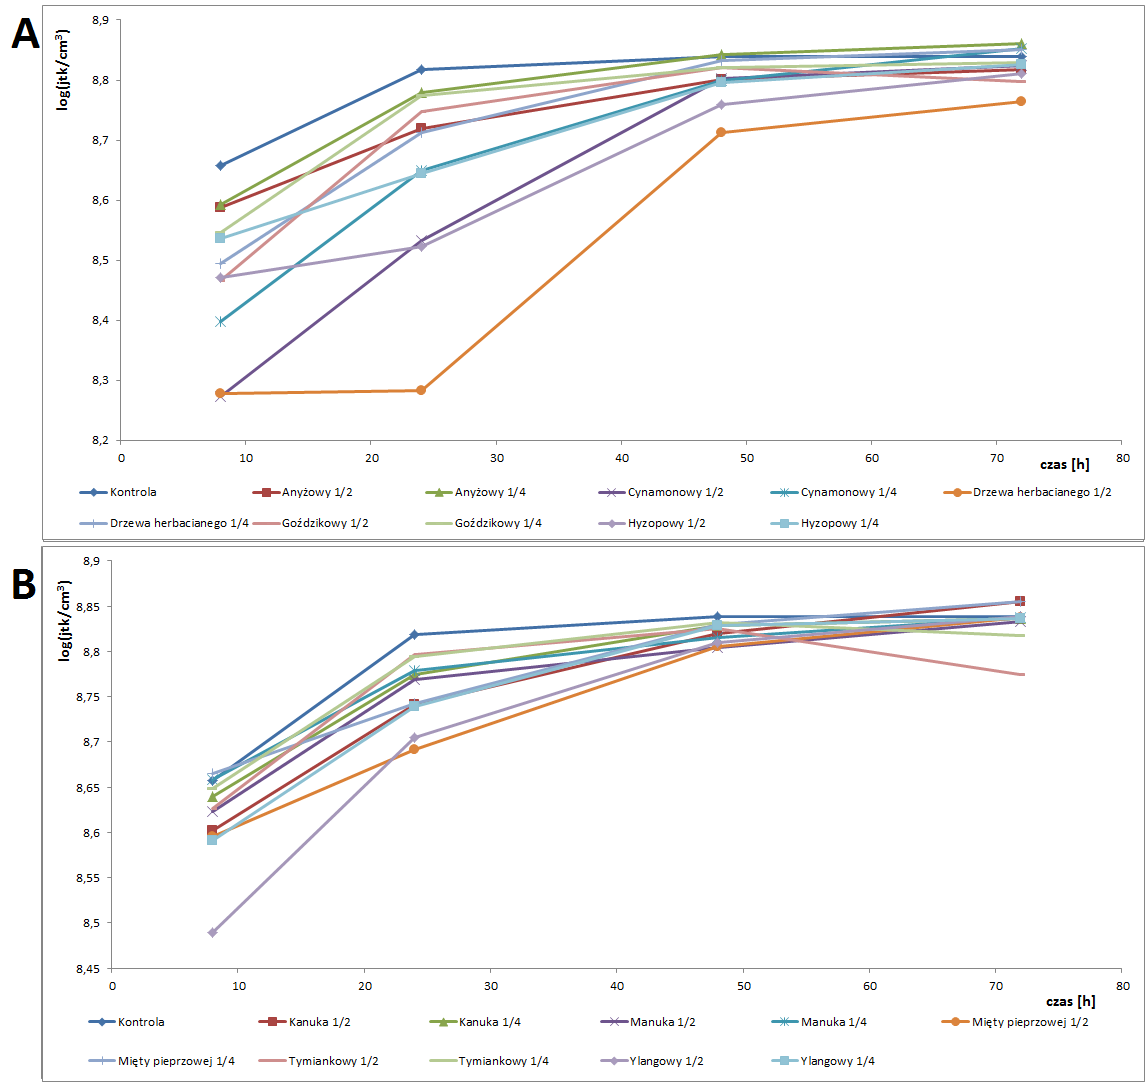
\includegraphics[scale=0.55]{img/dh2-c.png}
\caption{Dynamika tworzenia biofilmu bakterii \textit{Pseudomonas cedrina} DH2 w obecności olejków w stężeniu odpowiadającemu 1/2 oraz 1/4 MIC; A - olejek anyżowy, cynamonowy, drzewa herbacianego, goździkowy i hyzopowy, B - olejek kanuka, manuka, mięty pieprzowej, tymiankowy i ylangowy.}\label{dh2-c}
\end{center} 
\end{figure}

\clearpage

\chapter{Dyskusja}

Wywołane przez mikroflorę gospodarza oraz przez mikroflorę egzogenną infekcje bakteryjne są największą grupą zakażeń szpitalnych, co stanowi poważny problem w tych placówkach. Organizmy patogenne mogą rozwijać się w wielu miejscach na terenie szpitala - na sprzęcie medycznym, wyposażeniu sal, w wodzie czy powietrzu. Aby zapobiegać rozwojowi tych drobnoustrojów stosuje się detergenty i antybiotyki, lecz takie działanie może sprzyjać rozwojowi mikroorganizmów lekoopornych. 
W związku z tym od kilku lat poszukuje się alternatywnych, skutecznych środków hamujących rozwój patogenów. Środkami tymi, ze względu na swoje działanie przeciwdrobnoustrojowe mogą stać się olejki eteryczne\cite{zakszpit16, czaczyk}.

Olejki eteryczne dodawane do hodowli bakterii gram-ujemnych w odpowiednim stężeniu skutecznie hamują rozwój biofilmu, co potwierdza w swoich badaniach Małgorzata Gniewosz\cite{manukaikanuka}na przykładzie olejku manuka i kanuka, czy Yong-Guy Kim\cite{kim} przedstawiający wpływ olejku cynamonowego na biofilm bakterii \textit{Pseudomonas aeruginosa}.  
Analizując działanie bakteriobójcze olejków należy wziąć pod uwagę również fakt, iż minimalne stężenia hamujące mogą działać drażniąco na organizm człowieka, co w przypadku środowisk szpitalnych uniemożliwiałoby ich zastosowanie. 
W walce z zakażeniami szpitalnymi ważna jest nie tyle całkowita eradykacja, lecz utrzymanie ilości niepożądanych mikroorganizmów poniżej określonego poziomu \cite{zakszpit16}. 
Prowadzone badania stanowiły poszukiwania niższego niż wartość MIC stężenia olejku, które jednocześnie w wystarczającym stopniu hamowałoby rozwój biofilmu bakteryjnego na powierzchni medycznych cewników oddechowych.

Silne działanie hamujące rozwój niemal wszystkich spośród badanych szczepów bakterii wykazywał olejek drzewa herbacianego. Podobne spostrzeżenia w swoim atykule dokumentuje Aleksandra Garbusińska i wsp.\cite{drzewo1, drzewo2}. Szeroka gama mikroorganizmów, w tym bakterie gram-ujemne wykazują się dużą wrażliwością wobec niskich stężeń tego olejku. Wynika to ze sposobu w jaki olejek oddziałuje na komórki biofilmu - niszcząc ich błony biologiczne.

\clearpage
.

%drzewo1: http://www.czytelniamedyczna.pl/3544,przeglad-badan-in-vitro-oceniajacych-aktywnosc-przeciwdrobnoustrojowa-olejku-z-d.html
%drzewo2: http://www.czytelniamedyczna.pl/3868,aktywnosc-przeciwdrobnoustrojowa-olejku-z-drzewa-herbacianego-tea-tree-oil-w-bad.html

%nurt badawczy
% bartoszewicz: http://kpbc.umk.pl/Content/44547/01_Bartoszewicz.pdf
%kim: cinamon biofilm polym w:LITERATURA
%Bakterie gram-ujemne, dzięki swoim rozbudowanym mechanizmom oporności stanowią poważny problem w środowisku szpitalnym \cite{zakszpit16}.

\clearpage

\chapter{Wnioski i stwierdzenia końcowe}

\begin{itemize}
\item Olejek miętowy hamuje wzrost biofilmu wszystkich badanych szczepów bakterii na powierzchni cewników oddechowych PCV.

\item Wzrost biofilmu szczepów \textit{Pseudomonas aeruginosa} ATCC 15442, CFII i CFV oraz szczepu \textit{Pseudomonas cedrina} DH2 hamuje olejek miętowy, hyzopowy w stężeniu odpowiadającym 1/2 wartości MIC oraz olejek drzewa herbacianego w stężeniu 1/4 MIC.

\item Spowalniająco na rozwój biofilmu w hodowlach szczepu \textit{Pseudomonas cedrina} PC działał olejek tymiankowy, zaś w hodowlach szczepu \textit{Pseudomonas cedrina} DH1 olejek drzewa herbacianego oraz olejek anyżowy i goździkowy w stężeniu odpowiadającemu 1/2 wartości MIC.

\item Dodatek olejku ylangowego stymuluje wzrost biofilmu bakterii \textit{Pseudomonas aeruginosa} CFII i CFV, oraz \textit{Pseudomonas cedrina} PC.

\item Stymulująco na wzrost biofilmu bakterii \textit{Pseudomonas aeruginosa} CFII działa również olejek kanuka, na wzrost bakterii \textit{Pseudomonas aeruginosa} CFV - olejek kanuka, manuka oraz cynamonowy.

\item Na rozwój planktonu bakterii szczepu \textit{Pseudomonas aeruginosa} ATCC 15442 hamująco działa olejek mięty pieprzowej, zarówno w stężeniu 1/2 jak i 1/4 wartości MIC.

\item Widoczne spowolnienie rozwoju biomasy planktonu stwierdzono również dla szczepów  \textit{Pseudomonas aeruginosa} CFV i \textit{Pseudomonas cedrina} PC po dodaniu olejku drzewa herbacianego w stężeniu 1/4 MIC.

\end{itemize}


\clearpage

% bibliografia 
\bibliography{Praca2}
\bibliographystyle{plplain}

\listoffigures
\listoftables

\end{document}
